\documentclass[11pt]{book}
\usepackage[a4paper,margin=1in,headheight=16pt]{geometry}
\usepackage[T1]{fontenc}
\usepackage{lmodern}
\usepackage{microtype}
\usepackage{graphicx}
\usepackage{xcolor}
\usepackage{booktabs}
\usepackage{tabularx}
\usepackage{longtable}
\usepackage{array}
\usepackage{enumitem}
\usepackage{listings}
\usepackage[most]{tcolorbox}
\usepackage{fancyhdr}
\usepackage{titlesec}
\usepackage{hyperref}
\usepackage{float}
\usepackage{lastpage}
\usepackage{hyperref}
\usepackage{indentfirst}
\usepackage{forest}
\usepackage{seqsplit}
\usepackage{adjustbox}

\newcommand{\error}[1]{\texttt{\seqsplit{#1}}}
\newcommand{\code}[1]{\texttt{#1}}
\makeatletter

\renewcommand{\chaptermark}[1]{%
    \if@mainmatter
        \markboth{\@chapapp\ \thechapter.\ #1}{}
    \else
        \markboth{#1}{}
    \fi
}

\makeatother
\definecolor{hobbyblue}{HTML}{145DA0}
\definecolor{hobbydark}{HTML}{12344D}
\definecolor{codebackground}{HTML}{F5F7F9}
\definecolor{codeframe}{HTML}{D5DCE3}
\definecolor{notebackground}{HTML}{F1F6FB}
\definecolor{noteframe}{HTML}{4A90C2}
\definecolor{warningbackground}{HTML}{FFF8E6}
\definecolor{warningframe}{HTML}{C98A00}
\definecolor{tipbackground}{HTML}{EEF8F1}
\definecolor{tipframe}{HTML}{4B9560}

\lstdefinelanguage{HobbySpark}{sensitive=true,morekeywords={if,elif,else,while,for,in,True,False,None,break,continue,return,class,def,and,or,not,print,range,ActiveBuzzer, Led, on, wait, off},morecomment=[l]\#,morestring=[b]",morestring=[b]'}

\lstdefinestyle{tracebacks}{
	basicstyle=\ttfamily\small,
	literate={'}{{'}}1
}

\lstset{
	language=HobbySpark,
	backgroundcolor=\color{codebackground},
	basicstyle=\ttfamily\small,
	keywordstyle=\color{hobbyblue}\bfseries,
	stringstyle=\color{purple},
	commentstyle=\color{gray}\itshape,
	frame=single,
	rulecolor=\color{codeframe},
	numbers=left,
	numberstyle=\tiny\color{gray},
	numbersep=8pt,
	breaklines=true,
	keepspaces=true,
	showspaces=false,
	showstringspaces=false,
	columns=fullflexible,
	tabsize=4
}
\newtcolorbox{notebox}{breakable,colback=notebackground,colframe=noteframe,title=Note,fonttitle=\bfseries}
\newtcolorbox{tipbox}{breakable,colback=tipbackground,colframe=tipframe,title=Tip,fonttitle=\bfseries}
\newtcolorbox{warningbox}{breakable,colback=warningbackground,colframe=warningframe,title=Warning,fonttitle=\bfseries}



\pagestyle{fancy}
\fancyhf{}
\fancyhead[L]{\nouppercase{\leftmark}}
\fancyhead[R]{HobbySpark User Guide}
\fancyfoot[C]{\thepage}
\renewcommand{\headrulewidth}{0.4pt}
\fancypagestyle{plain}{
	\fancyhf{}
	\fancyhead[L]{\nouppercase{\leftmark}}
	\fancyhead[R]{HobbySpark User Guide}
	\fancyfoot[C]{\thepage}
	\renewcommand{\headrulewidth}{0.4pt}
}

\makeatletter

\titleformat{\chapter}[display]
{\normalfont\bfseries\color{hobbydark}}
{\filleft\Large\@chapapp\ \thechapter}
{10pt}
{\Huge}

\makeatother
\titleformat{\section}{\normalfont\Large\bfseries\color{hobbydark}}{\thesection}{0.8em}{}
\titleformat{\subsection}{\normalfont\large\bfseries\color{hobbydark}}{\thesubsection}{0.8em}{}
\setlist[itemize]{itemsep=2pt,topsep=4pt}
\setlist[enumerate]{itemsep=3pt,topsep=4pt}

\hypersetup{
	colorlinks=true,
	linkcolor=hobbyblue,
	urlcolor=hobbyblue,
	citecolor=hobbyblue,
	pdftitle={HobbySpark User Guide},
	pdfauthor={Arhanth}
}

\title{\Huge\bfseries HobbySpark\\[0.3em]\Large User Guide}
\author{Arhanth}
\date{\today}

\begin{document}
\frontmatter
	\begin{titlepage}

\newgeometry{top=1in,bottom=1in,right=0.75in,left=0.75in}

\begin{tikzpicture}[overlay,remember picture]
    \draw[line width=1.5pt]
        ($ (current page.north west) + (1.0cm,-1.0cm) $)
        rectangle
        ($ (current page.south east) + (-1.0cm,1.0cm) $);
\end{tikzpicture}

\begin{center}

    \vspace*{1.0cm}

    % HobbySpark logo
    
\includegraphics[width=0.5\textwidth]{images/icon.png}

    \vspace{0.8cm}

    % Main title
    {\Huge\bfseries HobbySpark}

    \vspace{0.3cm}

    {\LARGE\bfseries User Guide and Developer Reference}

    \vspace{0.7cm}

    % Description
    {\large
    \textit{
        A Comprehensive Guide to Programming, Configuring,\\
        and Extending the HobbySpark Framework
    }}

    \vspace{1.2cm}

    % Edition / version
    {\large\textbf{Version 1.0.0}}

    \vspace{0.25cm}

    {\large\textit{\today}}

	\vspace{0.25cm}

	{\Large\textit{Compiled by \LaTeX}}
    \vfill

    % Author
    {\large\textbf{Written by}}

    \vspace{0.25cm}

    {\Large\bfseries Arhanth}

    \vspace{1.2cm}

    % Closing statement
    {\small
    \textit{
        Documentation for the HobbySpark framework
    }}

\end{center}

\restoregeometry

\end{titlepage}
	\tableofcontents
	\newpage
	\listoffigures
	\newpage
	\listoftables
	\newpage
	\chapter*{Copyright and License}
\addcontentsline{toc}{chapter}{Copyright and License}

\vspace*{1cm}

\begin{center}
    {\Large\bfseries HobbySpark User Guide}

    \vspace{0.4cm}

    {\large Version 1.0.0}

    \vspace{0.8cm}

    {\large Copyright \textcopyright\ 2026 Arhanth}

    \vspace{1cm}
\end{center}

\section*{Copyright}

This documentation, including its text, examples, diagrams, tables, and
other original content, is copyright \textcopyright\ 2026 Arhanth.

HobbySpark and the accompanying documentation are provided as a project
for learning, development, experimentation, and educational use.

Except where otherwise stated, the contents of this documentation may not
be reproduced, redistributed, or modified for commercial purposes without
prior permission from the copyright holder.

\vspace{0.5cm}

\section*{License}

This documentation is released under the
\textbf{Creative Commons Attribution--NonCommercial 4.0 International
License (CC BY-NC 4.0)}.

Under this license, you are free to:

\begin{itemize}
    \item \textbf{Share} --- copy and redistribute the material in any
    medium or format.
    
    \item \textbf{Adapt} --- remix, transform, and build upon the material.
\end{itemize}

The following conditions apply:

\begin{itemize}
    \item \textbf{Attribution} --- appropriate credit must be given to
    Arhanth, a link to the license must be provided, and any changes made
    must be indicated.
    
    \item \textbf{NonCommercial} --- the material may not be used for
    commercial purposes.
\end{itemize}

The full terms of the license are available at:

\begin{center}
    \texttt{https://creativecommons.org/licenses/by-nc/4.0/}
\end{center}

\vspace{0.5cm}

\section*{Software License}

The license for the HobbySpark software itself may differ from the license
of this documentation. The licensing terms of the HobbySpark source code
take precedence over the terms stated here for the software.

\vfill

\begin{center}
    \textit{HobbySpark User Guide}\\
    \textit{Version 1.0.0}\\
    \textit{Written by Arhanth}
\end{center}
\newpage
	\mainmatter
	% !TeX root = ../main.tex
\chapter{Getting started}
\section{What is HobbySpark?}

HobbySpark is a programming language and development environment
designed for creating programs that interact with hardware such as
microcontroller boards and electronic components.

It provides a simple, readable programming language that lets you
write programs using familiar concepts such as variables, conditions,
loops, functions, and classes, while also providing classes designed
specifically for working with hardware.

Instead of requiring the user to deal directly with all of the
lower-level details of hardware programming, HobbySpark provides
higher-level objects and methods that represent the components being
used. This allows a program to describe what it wants the hardware to
do in a more natural way.

For example, a hardware component can be represented by an object:

\begin{lstlisting}
	led = Led(6)
\end{lstlisting}

The program can then interact with that object through its methods:

\begin{lstlisting}
	led.on()
	led.off()
\end{lstlisting}

HobbySpark is intended to make experimenting with electronics and
programming more approachable while still allowing users to build
increasingly complex projects.

\subsection{How HobbySpark Works}

From the user's point of view, the workflow is straightforward:

\begin{center}
	\textbf{Write your program}
	$\rightarrow$
	\textbf{Check it}
	$\rightarrow$
	\textbf{Build it}
	$\rightarrow$
	\textbf{Upload it}
	$\rightarrow$
	\textbf{Watch your hardware do something}
\end{center}

The user does not need to manually construct the underlying C++
program. HobbySpark handles the conversion required by its hardware
toolchain.

\subsection{What Can You Do with HobbySpark?}

HobbySpark programs can use ordinary programming features alongside
hardware-oriented functionality. This means the same language can be
used for both the logic of a program and the control of physical
hardware.

Some of the features available to HobbySpark programs include:

\begin{itemize}
	\item Variables
	\item \texttt{if}, \texttt{elif}, and \texttt{else} conditionals
	\item \texttt{while} and \texttt{for} loops(for loops only applicable for range)
	\item Functions
	\item Classes with constructors and operator overloading(with explicit return types)
	\item All python basic types (\texttt{bool}, \texttt{int}, \texttt{float} and \texttt{str})
	\item \texttt{break} and \texttt{continue}
	\item Programs that continuously interact with connected
	hardware
\end{itemize}

The goal of HobbySpark is simple: write code, connect hardware, and
make something happen.

\section{Requirements}
You will need the following:
\begin{enumerate}
	\item \textbf{Computer}
	\item \textbf{Applicable USB cable}
	\item \textbf{HobbySpark app}
	\item \textbf{Board}
	\item \textbf{The required devices like LEDs, motors, and sensors}
\end{enumerate}

	% !TeX root = ../main.tex
\chapter{Installation}
\section{Introduction}
In this chapter, we will install and complete the installation of HobbySpark and all of its dependencies.
You will need an internet connection and enough space for the app to be installed (Do not worry about disk space, HobbySpark is in mere megabytes). 

\section{Installing HobbySpark}
\begin{notebox}
	HobbySpark is supported currently for all the 3 mainstream operating systems-- Windows, Debian Linux, and MacOS. However, this documentation explains the installation procedure for windows only.
	\begin{itemize}
		\item The Linux install procedure is quite straight-forward, which you can easily follow.
		\item MacOS may be a bit trickier though, as HobbySpark is an open-source application. A open-source app can be licensed and notorised by Apple. Hoever, we haven't licensed and notorised  our app. However, you can follow the website's FAQ page and there will be instructions for how to install the app for MacOS 
	\end{itemize}
\end{notebox}

First, visit \href{https://sites.google.com/view/hobbyspark/downloads/windows}{here} and go down to the installer download button. Click the button. Once the download is finished, run the installer.

Now, you should probably see something close to Fig~\ref{fig:bsod}. {\Large Do not panic}, this is normal behavior, as HobbySpark does not have a software license from microsoft. Therefore, Windows does not know that there is an app called this, so it warns you that ithas an unverified publisher. As long as the app is from the real genuine repo or the genuine website, it's safe to press \code{more info} and then \code{run anyway}.
\begin{figure}[H]
	\centering
	\caption{The windows smart-screen}
	\label{fig:bsod}
	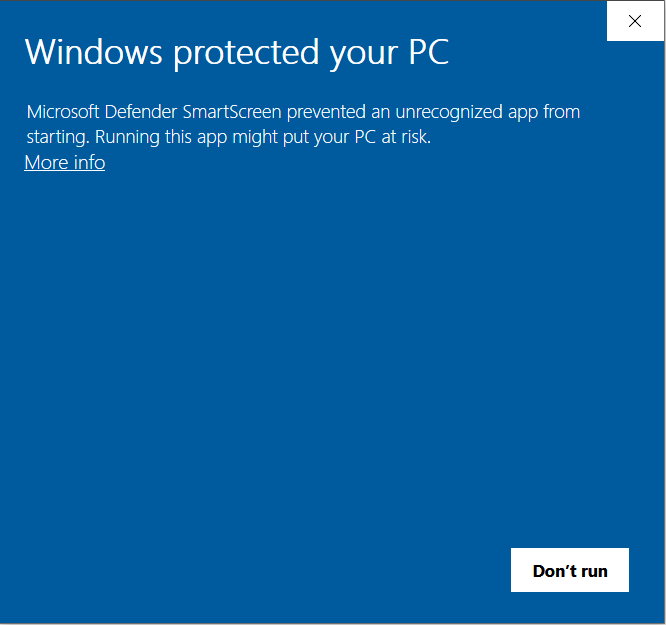
\includegraphics[scale=0.3]{images/bsod.png}
\end{figure}
\newpage
\subsection{Starting it up}
Now, once you click \code{run anyway}, the installer will ask you to choose the language for the installation process\emph{only}, so the app will be in English no matter what language you choose for installation.

\subsection{License agreement}
Now a license agreement page will show up. For your information, HobbySpark uses the Apache version 2.0 license. For those who don't know about it are free to read it. After doing that, click \code{I accept the agreement}.

\subsection{Important info and additional steps}
Now, it'll show you what you can do with HobbySpark as a short introduction. Next, it shows a window with a checkbox. You can check it if you want a desktop shortcut for HobbySpark.

\subsection{Actual installation}
Now it'll show you the various settings you have chosen, which should be similar to--
\begin{lstlisting}[style=tracebacks]
	Additional tasks:
	Additional shortcuts:
	Create a desktop shortcut
\end{lstlisting}


Next, you can press install. You will see a progress-bar. You can be sure the installation is almost finished when language names start appearing above the progress-bar. Next press finish and optionally check \code{Launch} to open HobbySpark immediately. 
\section{After installation}
Depending on whether you have some apps or not, you may or may not get a window to install Python and Arduino-cli. If these show up, follow the steps on the screen. Also, it may take a few moments for the app to open the first time as it installs some dependencies internally.

The first time you check or upload, it may pop up with a window saying that HobbySpark is installing some dependencies. These are Arduino frameworks. Please wait until the installation is complete. 

An internet connection will be required when you open the app for the first time, even if through the installer, or it may even end you up with an error.
	% !TeX root = ../main.tex 
\chapter{The HobbySpark interface}
\section{The main window}
The main window of HobbySpark is shown in Fig~\ref{fig:window}.
\begin{figure}[H]
	\centering
	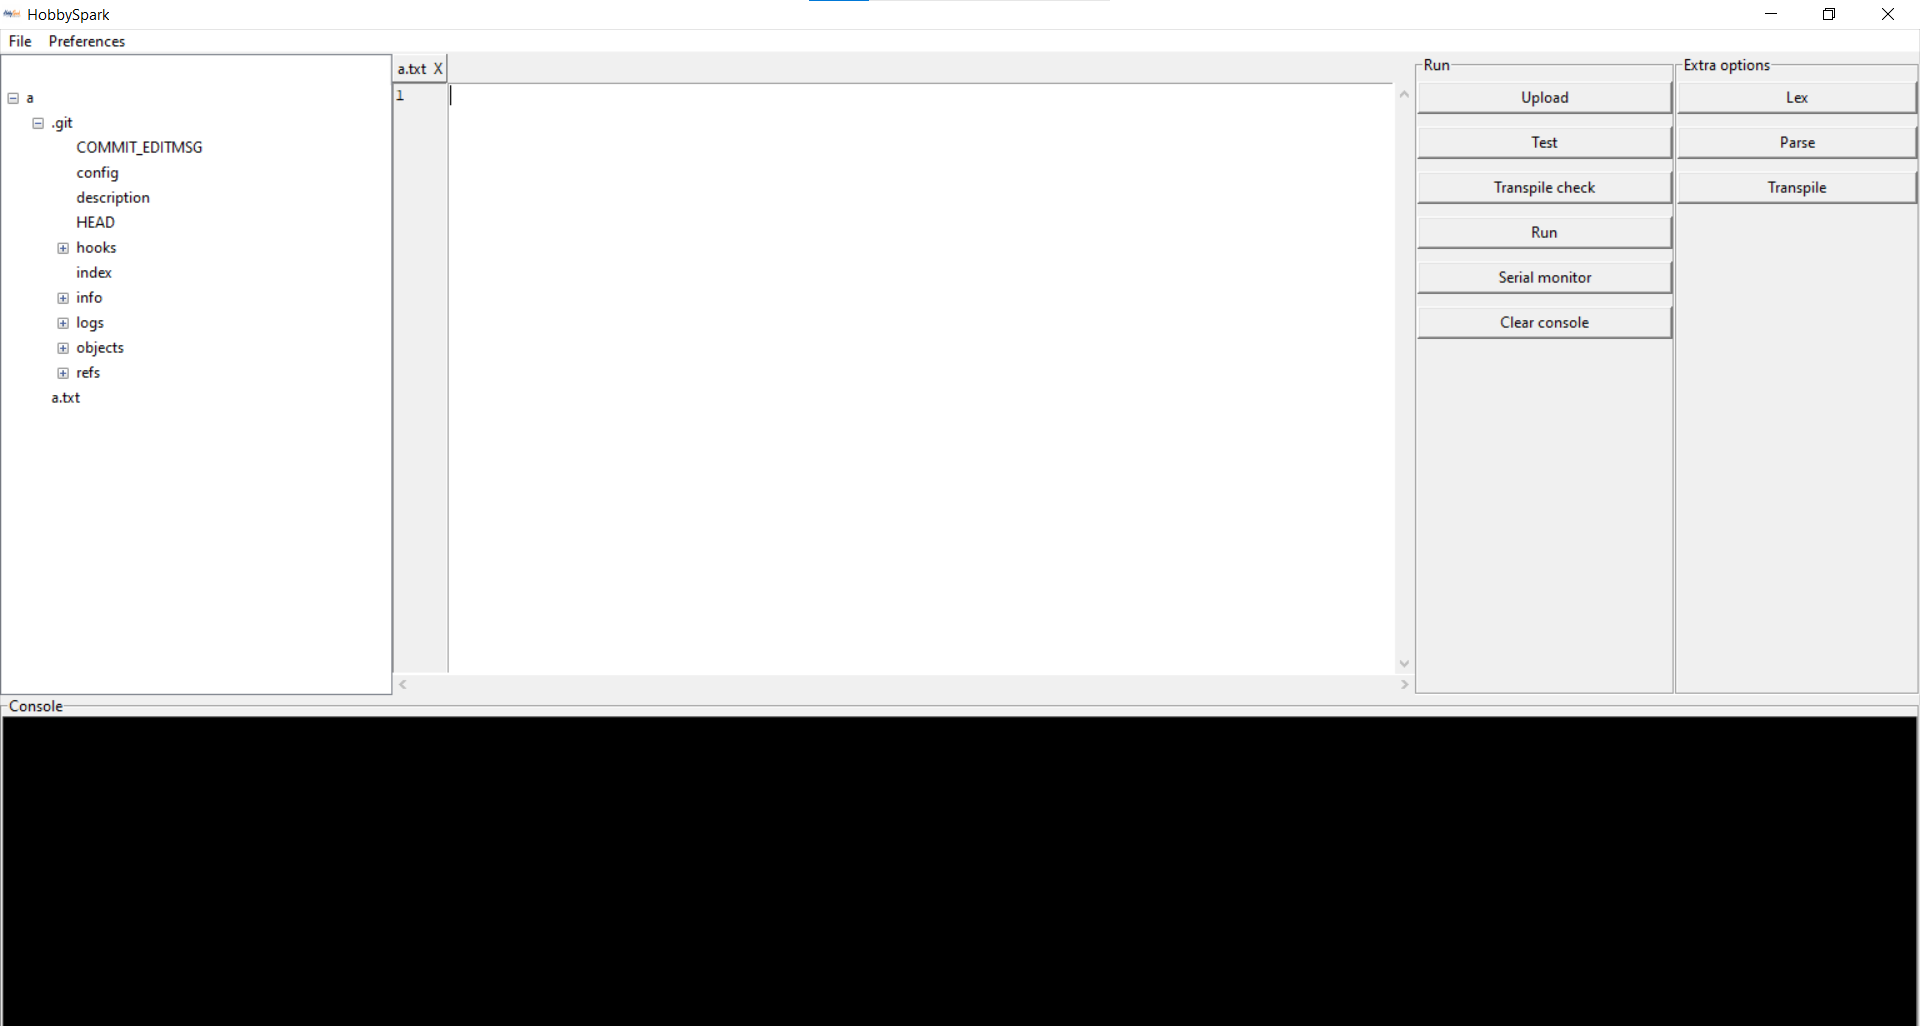
\includegraphics[scale=0.4]{images/main.png}
	\caption{The main window of HobbySpark}
	\label{fig:window}
\end{figure} 




All the buttons and their uses are explained below.

\subsection{Upload}
Uploads the code to the microcontroller, after asking board name and COM port.
\subsection{Test}
Goes through the whole process until compilation; it does not upload. The board name however will be asked.
\subsection{Transpile check}
Tests the program out until transpilation step. Will not ask anything.
\subsection{Run}
Runs the script using the standard \texttt{python filename}. Will not ask anything.
\subsection{Serial monitor}
Opens the serial monitor in a \emph{separate} window, after asking board name, COM port and baudrate.
\subsection{Clear console}
Clears the console.

\subsection{Lex}
Tokenizes the program completely and gives the token list as output for curious users.
\subsection{Parse}
Opens a new window that shows the whole program structure in a tree like structure.
\subsection{Transpile}
Transpiles and shows the complete transpiled C++ code.

\section{Interesting features}
\subsection{Birthday wishing}
\textcolor{red}{YES}, HobbySpark has a builtin birthday wishing system. It features a small window popup and playing of a non-copyrighted "Happy Birthday To You" song.
\subsection{Auto board and COM port fill-up}
Tired of selecting boards and COM ports? Well, fear no more cause we have a file called \texttt{settings.json} in which you can put the default COM port and board. Note that while putting the default values, the value should match exactly to what you get in the drop-down menu, or it may crash unexpectedly.

\section{Menus}
The \texttt{file} menu may be used to create new projects and also open existing ones. A new project in HobbySpark is any folder with the following files/folders:
\begin{itemize}
	\item .src/main.py
	\item COMPILATION/main.py/main.py.ino
	\item COMPILATION/main.py/package.h
	\item settings.json
\end{itemize}


Also note that the COMPILATION directory is auto-generated \emph{after} at least 1 test or upload process has been completed without errors.
\newpage
\section{A note on internal errors}
\begin{figure}[H]
	\centering
	\caption{An internal error that happened} 
	\label{fig:err}
	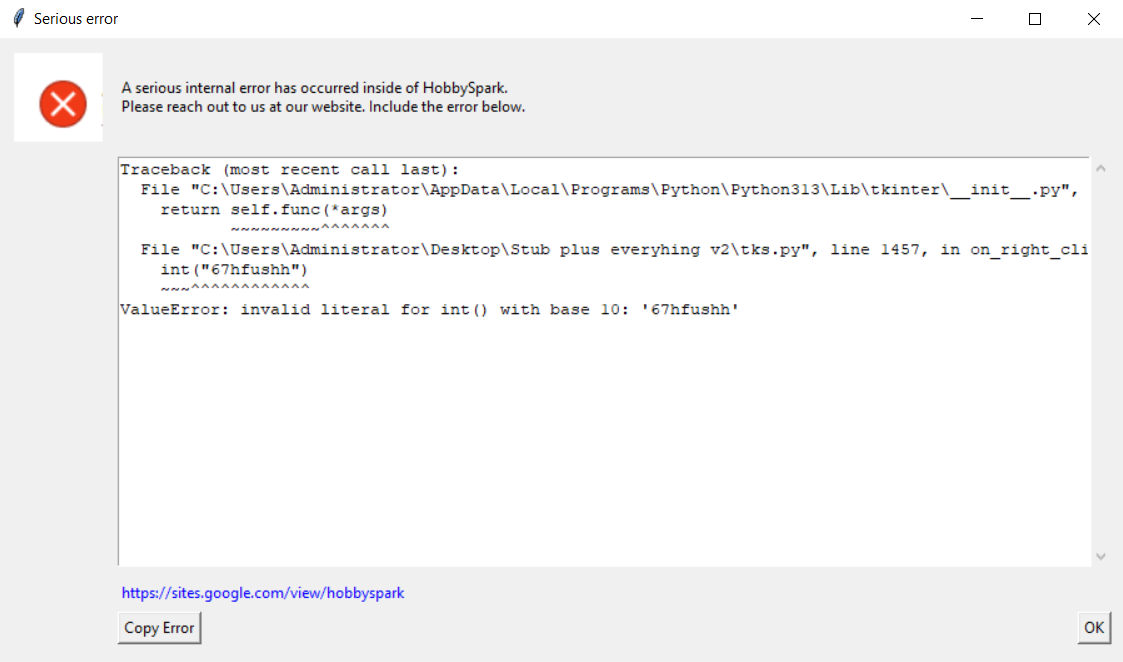
\includegraphics[scale=0.7]{images/error.png}
\end{figure}
While playing around with HobbySpark, if you see something like Fig~\ref{fig:err}, then you should probably do the steps shown on screen. HobbySpark is a developing open-source project. In the first version, the UI may not be stable. Therefore, we have put a safety guard that can watch for errors and report them to the user, so that they can write an issue to us, and we can resolve it.

	% !TeX root = ../main.tex
\chapter{User side framework}
\section{Introduction}
We have learnt about the GUI, but what about the actual code? This chapter fully explains the HobbySpark API so that you can write code that actually \emph{works}.

\section{A brief note on syntax}
\label{sec:syn}
The syntax of HobbySpark code is intentionally very close to Python. However, only the following features of Python are included in HobbySpark v1.0.0:
\begin{itemize}
	\item Variables (note that type annotations do not work, types are either semantically found out or the variable type is put as \code{auto} while generation of \code{C++} code)
	\item \texttt{if}, \texttt{elif}, and \texttt{else} conditionals
	\item \texttt{while} and \texttt{for} loops (for loops are \emph{only} applicable for range)
	\item Functions
	\item Classes with constructors and operator overloading (with explicit return types, which is not required in normal Python, but it is a HobbySpark specific )
	\item All the basic Python types (\texttt{bool}, \texttt{int}, \texttt{float} and \texttt{str})
	\item \texttt{break} and \texttt{continue}
\end{itemize}
\begin{warningbox}
	HobbySpark doesn't support all Python features. So writing code with features HobbySpark does not support may end up giving you an error.
\end{warningbox}

\section{Classes and Hardware Objects}

HobbySpark uses classes to represent hardware devices and other
reusable objects. Each class provides methods for interacting with
the corresponding device.

\newpage

\subsection{ActiveBuzzer}

Standard class for programming active buzzers.\\
It requires one argument:

\begin{enumerate}
	\item \texttt{pin} --- The pin connected to the active buzzer.
\end{enumerate}

Example usage:

\begin{lstlisting}
	buzzer = ActiveBuzzer(4)
	
	buzzer.on()
	
	wait(1)
	
	buzzer.off()
\end{lstlisting}

Methods:

\begin{tabular}{ll}
	\toprule
	\textbf{Method} & \textbf{Purpose}\\
	\midrule
	\texttt{on()} & Turns the buzzer on.\\
	\texttt{off()} & Turns the buzzer off.\\
	\texttt{toggle()} & Toggles the buzzer state.\\
	\texttt{return\_state()} & Returns the current buzzer state.\\
	\bottomrule
\end{tabular}





\subsection{Button}

Standard class for programming buttons.\\
It requires one argument:

\begin{enumerate}
	\item \texttt{pin} --- The pin connected to the button.
\end{enumerate}

Example usage:

\begin{lstlisting}
	button = Button("2")
	def on_press():
        pass
        # Put your code here
	button.when_read(on_pressed)
\end{lstlisting}

Methods:

\begin{tabular}{ll}
	\toprule
	\textbf{Method} & \textbf{Purpose}\\
	\midrule
	\texttt{read()} & Returns the current button state.\\
	\texttt{when\_read(func)} & Runs the supplied function whenever the button reading is true.\\
	\bottomrule
\end{tabular}




\newpage

\subsection{I2C\_LCD\_Display}

Class for controlling an I2C LCD display.\\
It requires four arguments and accepts a fifth argument, an optional address, which if not given, will be evaluated as the address \code{0x240}:

\begin{enumerate}
	\item \texttt{sda} --- The SDA pin.
	\item \texttt{scl} --- The SCL pin.
	\item \texttt{width} --- The display width.
	\item \texttt{height} --- The display height.
	\item \texttt{address} --- The I2C address of the display.
\end{enumerate}

Example usage:

\begin{lstlisting}
	display = I2C_LCD_Display(21, 22, 16, 2)
	
	display.set_cursor(0, 0)
	
	display.write("Hello")
\end{lstlisting}


Methods:

\begin{tabular}{ll}
	\toprule
	\textbf{Method} & \textbf{Purpose}\\
	\midrule
	\texttt{write(string)} & Writes text to the display.\\
	\texttt{add(string, importance)} & Adds text to the scrolling message system.\\
	\texttt{set\_cursor(x, y)} & Sets the display cursor position.\\
	\texttt{scroll\_text(string, delay, unit)} & Scrolls text across the display.\\
	\texttt{scroll\_with\_millis(start\_string, delay, unit)} & Starts non-blocking scrolling using millisecond timing.\\
	\bottomrule
\end{tabular}


\subsection{Led}

Standard class for programming LEDs.\\
It requires one argument:

\begin{enumerate}
	\item \texttt{pin} --- The pin connected to the LED.
\end{enumerate}

Example usage:

\begin{lstlisting}
	led = Led(4)
	
	led.on()
	
	wait(1)
	
	led.off()
\end{lstlisting}

Methods:

\begin{tabular}{ll}
	\toprule
	\textbf{Method} & \textbf{Purpose}\\
	\midrule
	\texttt{on()} & Turns the LED on.\\
	\texttt{off()} & Turns the LED off.\\
	\texttt{toggle()} & Toggles the LED state.\\
	\texttt{returnState()} & Returns the current LED state.\\
	\texttt{blink(speed, unit, times)} & Blinks the LED.\\
	\texttt{fade(time, unit)} & Fades the LED.\\
	\bottomrule
\end{tabular}


\subsection{PassiveBuzzer}

Standard class for programming passive buzzers.\\
It requires one argument:

\begin{enumerate}
	\item \texttt{pin} --- The pin connected to the passive buzzer.
\end{enumerate}

Example usage:

\begin{lstlisting}
	buzzer = PassiveBuzzer(4)
	
	buzzer.write(440, 1, SEC)
\end{lstlisting}

Methods:

\begin{tabular}{ll}
	\toprule
	\textbf{Method} & \textbf{Purpose}\\
	\midrule
	\texttt{write(frequency, time, unit)} & Plays the specified frequency for the specified duration.\\
	\texttt{write\_note(frequency, time, unit)} & Plays the specified frequency for the specified duration.\\
	\bottomrule
\end{tabular}





\subsection{RGB}

The \texttt{RGB} class represents an RGB color value.\\
It requires three arguments:

\begin{enumerate}
	\item \texttt{r} --- The red component.
	\item \texttt{g} --- The green component.
	\item \texttt{b} --- The blue component.
\end{enumerate}

Example usage:

\begin{lstlisting}
	color = RGB(255, 0, 0)
	
	hash = color.hash()
\end{lstlisting}

Methods:

\begin{tabular}{ll}
	\toprule
	\textbf{Method} & \textbf{Purpose}\\
	\midrule
	\texttt{hash()} & Returns the RGB value as a hexadecimal color string.\\
	\bottomrule
\end{tabular}

\newpage
\subsection{RGBLed}

Standard class for programming RGB LEDs.\\
It requires three arguments:

\begin{enumerate}
	\item \texttt{r} --- The red channel pin.
	\item \texttt{g} --- The green channel pin.
	\item \texttt{b} --- The blue channel pin.
\end{enumerate}

Example usage:

\begin{lstlisting}
	led = RGBLed(3, 5, 6)
	
	led.set(100, 0, 0)
	
	wait(1)
	
	led.off()
\end{lstlisting}

Methods:

\begin{tabular}{ll}
	\toprule
	\textbf{Method} & \textbf{Purpose}\\
	\midrule
	\texttt{set(r,g,b)} & Sets the RGB channel values.\\
	\texttt{off()} & Turns the RGB LED off.\\
	\texttt{returnState()} & Returns the current RGB state.\\
	\texttt{blink(r,g,b,speed,unit,times)} & Blinks the RGB LED using the specified color.\\
	\texttt{fade(time,unit)} & Fades the RGB LED.\\
	\bottomrule
\end{tabular}


\subsection{SerialMoniter}

Standard class for communicating through the serial monitor.\\
It accepts an optional baud rate.

Example usage:

\begin{lstlisting}
	serial = SerialMoniter(9600)
	
	serial.print("Hello")
	
	reading = serial.input()
\end{lstlisting}

Methods:

\begin{tabular}{ll}
	\toprule
	\textbf{Method} & \textbf{Purpose}\\
	\midrule
	\texttt{print(string)} & Prints data to the serial monitor.\\
	\texttt{input()} & Reads serial input.\\
	\texttt{available()} & Checks whether serial input is available.\\
	\bottomrule
\end{tabular}

\newpage
\subsection{ServoMotor}

Standard class for programming servo motors.\\
It requires one argument:

\begin{enumerate}
	\item \texttt{pin} --- The pin connected to the servo motor.
\end{enumerate}

Example usage:

\begin{lstlisting}
	servo = ServoMotor(9)
	
	servo.write(90)
\end{lstlisting}

Methods:

\begin{tabular}{ll}
	\toprule
	\textbf{Method} & \textbf{Purpose}\\
	\midrule
	\texttt{write(degrees)} & Moves the servo to the specified angle.\\
	\texttt{move\_smooth(degrees,speed,unit)} & Moves the servo smoothly toward the specified angle.\\
	\texttt{return\_state()} & Returns the current servo state.\\
	\bottomrule
\end{tabular}





\subsection{UltrasonicSensor}

Class for measuring distance using an ultrasonic sensor.\\
It requires two arguments:

\begin{enumerate}
	\item \texttt{trig} --- The trigger pin.
	\item \texttt{echo} --- The echo pin.
\end{enumerate}

Example usage:

\begin{lstlisting}
	sensor = UltrasonicSensor("6", "7")
	
	distance = sensor.distance()
	
	sensor.when_distance(10, close_object)
\end{lstlisting}

Methods:

\begin{tabular}{ll}
	\toprule
	\textbf{Method} & \textbf{Purpose}\\
	\midrule
	\texttt{distance()} & Returns the measured distance in centimeters.\\
	\texttt{when\_distance(distance,function)} & Executes the supplied function when the measured distance matches the specified distance.\\
	\bottomrule
\end{tabular}
\newpage
\section{Functions}

The HobbySpark framework provides functions for controlling the execution of a
program. These functions can be used to introduce delays while either allowing
or preventing the microcontroller from performing other operations.

\subsection{\texttt{wait()}}

The \texttt{wait()} function waits for a specified amount of time while allowing
background operations such as button reads and potentiometer reads to continue.

\begin{lstlisting}[language=Python]
wait(time, unit=MS) -> None
\end{lstlisting}

\textbf{Parameters:}

\begin{itemize}
    \item \texttt{time} -- The amount of time to wait. It must be an
    \texttt{int} or \texttt{float}.
    
    \item \texttt{unit} -- The unit in which \texttt{time} is specified.
    It must be an \texttt{int}. The default value is \texttt{MS}.
\end{itemize}

\textbf{Behaviour:}

Unlike a complete blocking delay, \texttt{wait()} allows operations such as
button reads and potentiometer reads to run during the waiting period.

\textbf{Errors:}

\begin{itemize}
    \item \texttt{InvalidArgumentError} is raised if \texttt{time} is not an
    \texttt{int} or \texttt{float}.
    
    \item \texttt{InvalidArgumentError} is raised if \texttt{unit} is not a
    \texttt{float}.
\end{itemize}


\subsection{\texttt{stop()}}

The \texttt{stop()} function completely blocks the microcontroller for the
specified amount of time. During this period, the microcontroller does not
perform other operations.

\begin{lstlisting}
stop(time, unit=MS) -> None
\end{lstlisting}

\textbf{Parameters:}

\begin{itemize}
    \item \texttt{time} -- The amount of time for which the microcontroller
    should be stopped. It must be an \texttt{int} or \texttt{float}.
    
    \item \texttt{unit} -- The unit in which \texttt{time} is specified.
    It must be an \texttt{int}. The default value is \texttt{MS}.
\end{itemize}

\textbf{Behaviour:}

The \texttt{stop()} function completely blocks the microcontroller for the
specified duration. Unlike \texttt{wait()}, other operations do not run during
this period.

\textbf{Errors:}

\begin{itemize}
    \item \texttt{InvalidArgumentError} is raised if \texttt{time} is not an
    \texttt{int} or \texttt{float}.
    
    \item \texttt{InvalidArgumentError} is raised if \texttt{unit} is not a
    \texttt{float}.
\end{itemize}

\newpage
\section{Constants}

The HobbySpark framework defines several constants that can be used
throughout a program for timing and musical-note frequencies.

\subsection{\texttt{MS}}



\texttt{MS} represents milliseconds. It has the value \texttt{1}, so a
value multiplied by \texttt{MS} remains in milliseconds.

For example:

\begin{lstlisting}
stop(500, MS)
\end{lstlisting}

pauses execution for 500 milliseconds.

\subsection{\texttt{SEC}}

\begin{lstlisting}[language=C++]
float SEC = 1000;
\end{lstlisting}

\texttt{SEC} represents seconds in milliseconds. Its value is
\texttt{1000}, because one second is equal to 1000 milliseconds.

For example:

\begin{lstlisting}[language=C++]
stop(2, SEC);
\end{lstlisting}

pauses execution for 2000 milliseconds, or two seconds.

\subsection{\texttt{US}}

\begin{lstlisting}[language=C++]
float US = 0.001;
\end{lstlisting}

\texttt{US} represents microseconds in the timing calculations used by
the framework. Its value is \texttt{0.001}.

\subsection{Musical Note Constants}

The HobbySpark framework provides frequency constants for musical notes
from octave 1 through octave 8. The values represent frequencies in
hertz and can be supplied to functions that generate tones.

The note constants are provided as follows:

\begin{enumerate}
    \item \texttt{NOTE\_C1} -- C in octave 1, 32.70 Hz.
    \item \texttt{NOTE\_CS1} -- C-sharp in octave 1, 34.65 Hz.
    \item \texttt{NOTE\_DF1} -- D-flat in octave 1; an alias of \texttt{NOTE\_CS1}.
    \item \texttt{NOTE\_D1} -- D in octave 1, 36.71 Hz.
    \item \texttt{NOTE\_DS1} -- D-sharp in octave 1, 38.89 Hz.
    \item \texttt{NOTE\_EF1} -- E-flat in octave 1; an alias of \texttt{NOTE\_DS1}.
    \item \texttt{NOTE\_E1} -- E in octave 1, 41.20 Hz.
    \item \texttt{NOTE\_F1} -- F in octave 1, 43.65 Hz.
    \item \texttt{NOTE\_FS1} -- F-sharp in octave 1, 46.25 Hz.
    \item \texttt{NOTE\_GF1} -- G-flat in octave 1; an alias of \texttt{NOTE\_FS1}.
    \item \texttt{NOTE\_G1} -- G in octave 1, 49.00 Hz.
    \item \texttt{NOTE\_GS1} -- G-sharp in octave 1, 51.91 Hz.
    \item \texttt{NOTE\_AF1} -- A-flat in octave 1; an alias of \texttt{NOTE\_GS1}.
    \item \texttt{NOTE\_A1} -- A in octave 1, 55.00 Hz.
    \item \texttt{NOTE\_AS1} -- A-sharp in octave 1, 58.27 Hz.
    \item \texttt{NOTE\_BF1} -- B-flat in octave 1; an alias of \texttt{NOTE\_AS1}.
    \item \texttt{NOTE\_B1} -- B in octave 1, 61.74 Hz.

    \item \texttt{NOTE\_C2} -- C in octave 2, 65.41 Hz.
    \item \texttt{NOTE\_CS2} -- C-sharp in octave 2, 69.30 Hz.
    \item \texttt{NOTE\_DF2} -- D-flat in octave 2; an alias of \texttt{NOTE\_CS2}.
    \item \texttt{NOTE\_D2} -- D in octave 2, 73.42 Hz.
    \item \texttt{NOTE\_DS2} -- D-sharp in octave 2, 77.78 Hz.
    \item \texttt{NOTE\_EF2} -- E-flat in octave 2; an alias of \texttt{NOTE\_DS2}.
    \item \texttt{NOTE\_E2} -- E in octave 2, 82.41 Hz.
    \item \texttt{NOTE\_F2} -- F in octave 2, 87.31 Hz.
    \item \texttt{NOTE\_FS2} -- F-sharp in octave 2, 92.50 Hz.
    \item \texttt{NOTE\_GF2} -- G-flat in octave 2; an alias of \texttt{NOTE\_FS2}.
    \item \texttt{NOTE\_G2} -- G in octave 2, 98.00 Hz.
    \item \texttt{NOTE\_GS2} -- G-sharp in octave 2, 103.83 Hz.
    \item \texttt{NOTE\_AF2} -- A-flat in octave 2; an alias of \texttt{NOTE\_GS2}.
    \item \texttt{NOTE\_A2} -- A in octave 2, 110.00 Hz.
    \item \texttt{NOTE\_AS2} -- A-sharp in octave 2, 116.54 Hz.
    \item \texttt{NOTE\_BF2} -- B-flat in octave 2; an alias of \texttt{NOTE\_AS2}.
    \item \texttt{NOTE\_B2} -- B in octave 2, 123.47 Hz.

    \item \texttt{NOTE\_C3} -- C in octave 3, 130.81 Hz.
    \item \texttt{NOTE\_CS3} -- C-sharp in octave 3, 138.59 Hz.
    \item \texttt{NOTE\_DF3} -- D-flat in octave 3; an alias of \texttt{NOTE\_CS3}.
    \item \texttt{NOTE\_D3} -- D in octave 3, 146.83 Hz.
    \item \texttt{NOTE\_DS3} -- D-sharp in octave 3, 155.56 Hz.
    \item \texttt{NOTE\_EF3} -- E-flat in octave 3; an alias of \texttt{NOTE\_DS3}.
    \item \texttt{NOTE\_E3} -- E in octave 3, 164.81 Hz.
    \item \texttt{NOTE\_F3} -- F in octave 3, 174.61 Hz.
    \item \texttt{NOTE\_FS3} -- F-sharp in octave 3, 185.00 Hz.
    \item \texttt{NOTE\_GF3} -- G-flat in octave 3; an alias of \texttt{NOTE\_FS3}.
    \item \texttt{NOTE\_G3} -- G in octave 3, 196.00 Hz.
    \item \texttt{NOTE\_GS3} -- G-sharp in octave 3, 207.65 Hz.
    \item \texttt{NOTE\_AF3} -- A-flat in octave 3; an alias of \texttt{NOTE\_GS3}.
    \item \texttt{NOTE\_A3} -- A in octave 3, 220.00 Hz.
    \item \texttt{NOTE\_AS3} -- A-sharp in octave 3, 233.08 Hz.
    \item \texttt{NOTE\_BF3} -- B-flat in octave 3; an alias of \texttt{NOTE\_AS3}.
    \item \texttt{NOTE\_B3} -- B in octave 3, 246.94 Hz.

    \item \texttt{NOTE\_C4} -- C in octave 4, 261.63 Hz.
    \item \texttt{NOTE\_CS4} -- C-sharp in octave 4, 277.18 Hz.
    \item \texttt{NOTE\_DF4} -- D-flat in octave 4; an alias of \texttt{NOTE\_CS4}.
    \item \texttt{NOTE\_D4} -- D in octave 4, 293.66 Hz.
    \item \texttt{NOTE\_DS4} -- D-sharp in octave 4, 311.13 Hz.
    \item \texttt{NOTE\_EF4} -- E-flat in octave 4; an alias of \texttt{NOTE\_DS4}.
    \item \texttt{NOTE\_E4} -- E in octave 4, 329.63 Hz.
    \item \texttt{NOTE\_F4} -- F in octave 4, 349.23 Hz.
    \item \texttt{NOTE\_FS4} -- F-sharp in octave 4, 369.99 Hz.
    \item \texttt{NOTE\_GF4} -- G-flat in octave 4; an alias of \texttt{NOTE\_FS4}.
    \item \texttt{NOTE\_G4} -- G in octave 4, 392.00 Hz.
    \item \texttt{NOTE\_GS4} -- G-sharp in octave 4, 415.30 Hz.
    \item \texttt{NOTE\_AF4} -- A-flat in octave 4; an alias of \texttt{NOTE\_GS4}.
    \item \texttt{NOTE\_A4} -- A in octave 4, 440.00 Hz.
    \item \texttt{NOTE\_AS4} -- A-sharp in octave 4, 466.16 Hz.
    \item \texttt{NOTE\_BF4} -- B-flat in octave 4; an alias of \texttt{NOTE\_AS4}.
    \item \texttt{NOTE\_B4} -- B in octave 4, 493.88 Hz.

    \item \texttt{NOTE\_C5} -- C in octave 5, 523.25 Hz.
    \item \texttt{NOTE\_CS5} -- C-sharp in octave 5, 554.37 Hz.
    \item \texttt{NOTE\_DF5} -- D-flat in octave 5; an alias of \texttt{NOTE\_CS5}.
    \item \texttt{NOTE\_D5} -- D in octave 5, 587.33 Hz.
    \item \texttt{NOTE\_DS5} -- D-sharp in octave 5, 622.25 Hz.
    \item \texttt{NOTE\_EF5} -- E-flat in octave 5; an alias of \texttt{NOTE\_DS5}.
    \item \texttt{NOTE\_E5} -- E in octave 5, 659.26 Hz.
    \item \texttt{NOTE\_F5} -- F in octave 5, 698.46 Hz.
    \item \texttt{NOTE\_FS5} -- F-sharp in octave 5, 739.99 Hz.
    \item \texttt{NOTE\_GF5} -- G-flat in octave 5; an alias of \texttt{NOTE\_FS5}.
    \item \texttt{NOTE\_G5} -- G in octave 5, 783.99 Hz.
    \item \texttt{NOTE\_GS5} -- G-sharp in octave 5, 830.61 Hz.
    \item \texttt{NOTE\_AF5} -- A-flat in octave 5; an alias of \texttt{NOTE\_GS5}.
    \item \texttt{NOTE\_A5} -- A in octave 5, 880.00 Hz.
    \item \texttt{NOTE\_AS5} -- A-sharp in octave 5, 932.33 Hz.
    \item \texttt{NOTE\_BF5} -- B-flat in octave 5; an alias of \texttt{NOTE\_AS5}.
    \item \texttt{NOTE\_B5} -- B in octave 5, 987.77 Hz.

    \item \texttt{NOTE\_C6} -- C in octave 6, 1046.50 Hz.
    \item \texttt{NOTE\_CS6} -- C-sharp in octave 6, 1108.73 Hz.
    \item \texttt{NOTE\_DF6} -- D-flat in octave 6; an alias of \texttt{NOTE\_CS6}.
    \item \texttt{NOTE\_D6} -- D in octave 6, 1174.66 Hz.
    \item \texttt{NOTE\_DS6} -- D-sharp in octave 6, 1244.51 Hz.
    \item \texttt{NOTE\_EF6} -- E-flat in octave 6; an alias of \texttt{NOTE\_DS6}.
    \item \texttt{NOTE\_E6} -- E in octave 6, 1318.51 Hz.
    \item \texttt{NOTE\_F6} -- F in octave 6, 1396.91 Hz.
    \item \texttt{NOTE\_FS6} -- F-sharp in octave 6, 1479.98 Hz.
    \item \texttt{NOTE\_GF6} -- G-flat in octave 6; an alias of \texttt{NOTE\_FS6}.
    \item \texttt{NOTE\_G6} -- G in octave 6, 1567.98 Hz.
    \item \texttt{NOTE\_GS6} -- G-sharp in octave 6, 1661.22 Hz.
    \item \texttt{NOTE\_AF6} -- A-flat in octave 6; an alias of \texttt{NOTE\_GS6}.
    \item \texttt{NOTE\_A6} -- A in octave 6, 1760.00 Hz.
    \item \texttt{NOTE\_AS6} -- A-sharp in octave 6, 1864.66 Hz.
    \item \texttt{NOTE\_BF6} -- B-flat in octave 6; an alias of \texttt{NOTE\_AS6}.
    \item \texttt{NOTE\_B6} -- B in octave 6, 1975.53 Hz.

    \item \texttt{NOTE\_C7} -- C in octave 7, 2093.00 Hz.
    \item \texttt{NOTE\_CS7} -- C-sharp in octave 7, 2217.46 Hz.
    \item \texttt{NOTE\_DF7} -- D-flat in octave 7; an alias of \texttt{NOTE\_CS7}.
    \item \texttt{NOTE\_D7} -- D in octave 7, 2349.32 Hz.
    \item \texttt{NOTE\_DS7} -- D-sharp in octave 7, 2489.02 Hz.
    \item \texttt{NOTE\_EF7} -- E-flat in octave 7; an alias of \texttt{NOTE\_DS7}.
    \item \texttt{NOTE\_E7} -- E in octave 7, 2637.02 Hz.
    \item \texttt{NOTE\_F7} -- F in octave 7, 2793.83 Hz.
    \item \texttt{NOTE\_FS7} -- F-sharp in octave 7, 2959.96 Hz.
    \item \texttt{NOTE\_GF7} -- G-flat in octave 7; an alias of \texttt{NOTE\_FS7}.
    \item \texttt{NOTE\_G7} -- G in octave 7, 3135.96 Hz.
    \item \texttt{NOTE\_GS7} -- G-sharp in octave 7, 3322.44 Hz.
    \item \texttt{NOTE\_AF7} -- A-flat in octave 7; an alias of \texttt{NOTE\_GS7}.
    \item \texttt{NOTE\_A7} -- A in octave 7, 3520.00 Hz.
    \item \texttt{NOTE\_AS7} -- A-sharp in octave 7, 3729.31 Hz.
    \item \texttt{NOTE\_BF7} -- B-flat in octave 7; an alias of \texttt{NOTE\_AS7}.
    \item \texttt{NOTE\_B7} -- B in octave 7, 3951.07 Hz.

    \item \texttt{NOTE\_C8} -- C in octave 8, 4186.01 Hz.
\end{enumerate}

		\chapter{Code Quirks}
	\section{Introduction}
	HobbySpark has some small interesting quirks that people can often miss. This chapter explains all of them.
	\section{Board selection}
	HobbySpark currently supports 30 different boards. Therefore, you \textbf{must} use a special function called \code{set\_board}. The usage is:
	\begin{lstlisting}
		set_board(BoardName(), debug)
	\end{lstlisting}
	The first argument is your board's name(ArduinoNano, ArduinoUnoR3, etc.) and the second one gives debug output similar to:
	\begin{lstlisting}
		Device: Led has run fade(time=1, unit=second\seconds(1000))
	\end{lstlisting}
	if the argument is true.
	
	\section{Package inclusion}
	The HobbySpark package isn't magically included by python. But you don't need to do the usual \code{python -m pip install package} because fortunately, the HobbySpark GUI automatically adds the package to the python PATH. You just need to put this line at the start--
	
	\begin{lstlisting}
		from stub import *
	\end{lstlisting}  
	
	Its tempting to do just \code{import}, but that will cause an error. Also, there are a few utilities that aren't defined in \code{C++}, which can cause an error. The parser blocks you from doing any plain imports.
	
	\newpage
	\section{Pin names}
	Pin names are just plain numbers if they are digital pins or plain numbers with an \code{A} prefixed to it. If you are accustomed to prefixing digital pins with a \code{D}, bad luck because unfortunately, HobbySpark completely rejects these and also throws a \code{InvalidPinTypeError}. Section~\ref{sec:pintyperror} explains the error and its meaning fully.
	
	\section{Opening projects}
	As soon as HobbySpark launches, you will see a file explorer thing that will ask you a directory, which will be the project directory. You can always change it in the menu. 
	
	Unlike other popular editors like VS-code and Sublime Text, HobbySpark doesn't remember paths. So, you'll unfortunately enter in your path again and again as you open the app.
    
		\chapter{Exceptions, explained}
	\section{Introduction}
	There are mainly 4 types of exceptions in HobbySpark:
	\begin{itemize}
		\item Syntax errors
		\item Transpilation errors
		\item Runtime errors
		\item Compile time error
	\end{itemize}
	
	Let us go through them carefully now:
	
	\section{Syntax errors}
	This error means that you haven't followed the correct syntax of python. For example:
	\begin{lstlisting}
		if :
		1234abcd
	\end{lstlisting}
	Causes a SyntaxError, or more verbosely--
	\begin{lstlisting}[style=tracebacks]
		Could not run:   File "<stdin>", line 1
		if :
		^
		SyntaxError: invalid syntax
	\end{lstlisting}
	
	\begin{notebox}
		Syntax errors may have very less info about \emph{what} really went wrong, but you can usually figure out what is the error. If you cannot seem to be able to do so, then spend your time with your favorite LLM trying to find out what's the actual problem.
	\end{notebox}
	\newpage
	\section{Transpilation errors}
	As explained in Section~\ref{sec:syn}, HobbySpark doesn't have all the features in python, so here comes transpilation errors. Transpilation errors happen when you use a feature not implemented in HobbySpark yet. For example:
	\begin{lstlisting}
		a = 23
		a+=1
	\end{lstlisting}
	Causes a UnsupportedNodeError, or more verbosely--
	\begin{lstlisting}[style=tracebacks]
		Failed to transpile code, 
		Node VariableCompAssignNode:
		op = ADD_COMPOUND
		left:
		VariableNameNode:
		name = a
		type = NUMBER
		right:
		NumberNode:
		value = 1
		is unsupported.
	\end{lstlisting}
	
	\begin{notebox}
		Transpilation errors don't mean you can't implement a feature, because there's always another feature that already does it, just in the long way. For example, the earlier code could be replaced with--
		\begin{lstlisting}
			a = 23
			a = a + 1
		\end{lstlisting}
		to not give any error.
	\end{notebox}
	
	\section{Runtime errors}
	This topic is very big, therefore, we will make a new chapter called Chapter~\ref{chap:run}
	
	\section{Compile time errors}
	These are errors that have come from the \code{C++} runtime. These usually don't happen. All the same, an example of error if you click yes after entering nothing for the \code{fqbn} asking prompt -- 
	\begin{lstlisting}
		Failed to compile, Missing FQBN (Fully Qualified Board Name)
	\end{lstlisting}
	\begin{tipbox}
		Compile errors clearly define what has happened, so it is easy for us to find what went wrong.
	\end{tipbox}
	\chapter{Runtime errors}
	\label{chap:run}
	\section{Introduction}
	Runtime errors are errors that happen before any parsing, lexing or transpiling ever happens. Python reports these errors and HobbySpark catches that report and in turn informs the user about it. There are many runtime errors already built onto python. All the predefined errors in python are given below: 
	\begin{itemize}
		\item \textbf{SyntaxError} -- The Python code does not follow valid syntax.
		\item \textbf{IndentationError} -- The indentation of the code is incorrect.
		\item \textbf{TabError} -- Tabs and spaces are mixed inconsistently for indentation.
		\item \textbf{NameError} -- A variable or name is used before it has been defined.
		\item \textbf{TypeError} -- An operation or function is used with an inappropriate type.
		\item \textbf{ValueError} -- A function receives the correct type but an invalid value.
		\item \textbf{IndexError} -- A sequence is accessed using an index that does not exist.
		\item \textbf{KeyError} -- A dictionary is accessed using a key that does not exist.
		\item \textbf{AttributeError} -- An object does not have the requested attribute or method.
		\item \textbf{ImportError} -- A requested module or name cannot be imported.
		\item \textbf{ModuleNotFoundError} -- The requested module cannot be found.
		\item \textbf{ZeroDivisionError} -- A number is divided by zero.
		\item \textbf{FileNotFoundError} -- A requested file or directory cannot be found.
		\item \textbf{PermissionError} -- The operation does not have sufficient permission.
		\item \textbf{RecursionError} -- The maximum recursion depth is exceeded.
		\item \textbf{MemoryError} -- The program cannot allocate enough memory.
		\item \textbf{RuntimeError} -- An error occurs that does not fit another specific category.
		\item \textbf{NotImplementedError} -- An operation or method has not been implemented.
		\item \textbf{AssertionError} -- An \texttt{assert} statement evaluates to false.
		\item \textbf{EOFError} -- Input is requested but the end of the input stream is reached.
		\item \textbf{KeyboardInterrupt} -- The user interrupts the program, usually with \texttt{Ctrl+C}.
		\item \textbf{SystemExit} -- The program requests that Python terminate execution.
		\item \textbf{UnboundLocalError} -- A local variable is referenced before it has been assigned a value.
		\item \textbf{StopIteration} -- An iterator has no more values to produce.
		\item \textbf{UnicodeError} -- A Unicode-related encoding or decoding operation fails.
	\end{itemize}
	However, there are still many HobbySpark specific errors, which are explained below:
	\section{PinNotApplicableError} 
	It means the pin you have given does not have the correct specifications for the use case. For example: 
	\begin{lstlisting} 
		from stub import * 
		set_board(ArduinoNano()) 
		led = Led("A1") 
		led.fade(1, SEC) 
	\end{lstlisting} 
	gives a error-- 
	\begin{lstlisting}[style=tracebacks] 
		Traceback (most recent call last): 
		File "<stdin>", line 4, in <module> 
		led.fade(1, SEC) 
		~~~~~~~~^^^^^^^^ 
		File "<stub path>", line 76, in fade 
		raise PinNotApplicableError(self.pin.pinname, "non PWM", "PWM") 
		stub.Errors.PinNotApplicableError: [Error number: 0.0.0]Error: An non PWM pin(A1) was used where PWM was needed. 
		Hint: Use a PWM pin for this device. 
		__________________________________________ 
		Remember, Errors are part of the process.  
		Each one helps you understand your code better. 
		Something went wrong -- that is okay. 
		Every error is a step toward a better program. 
		__________________________________________ 
		If the traceback worried you, do not worry, it will lead you to the exact place the error happend. 
		If the traceback ends with line numbers that are not yours they are usually just raise statements in the module. 
		__________________________________________ 
		
	\end{lstlisting} 
	
	It happens for: 
	\begin{enumerate} 
		\item PWM pin not given 
		\item Digital pin given where analog needed 
	\end{enumerate} 
	\newpage 
	
	\section{PinOutOfRangeError} 
	It means the pin you have given is outside the valid pin range of the current board. For example: 
	\begin{lstlisting} 
		from stub import * 
		set_board(ArduinoNano()) 
		led = Led("366") 
	\end{lstlisting} 
	gives an error-- 
	\begin{lstlisting}[style=tracebacks] 
		Traceback (most recent call last): 
		File "<stdin>", line 3, in <module> 
		led = Led("366") 
		File "<stdin>", line 40, in **init** 
		self.pin=Pin(pin,"both") 
		~~~^^^^^^^^^^^^ 
		File "<stdin>", line 102, in **init** 
		raise PinOutOfRangeError(pin,Boards.CURRENTBOARD) 
		stub.Errors.PinOutOfRangeError: [Error number: 0.0.1]Pin 366 was used when the valid pin range is 0-A7 
		__________________________________________ 
		Remember, Errors are part of the process. Each one helps you understand your code better. 
		Something went wrong -- that's okay. 
		Every error is a step toward a better program. 
		__________________________________________ 
		If the traceback worried you, don't worry, it will lead you to the exact place the error happend. 
		If the traceback ends with line numbers that are not yours they are usually just raise statements in the module. 
		__________________________________________ 
	\end{lstlisting} 
	
	
	It happens when: 
	\begin{enumerate} 
		\item A pin name outside the valid range of the current board is given. 
	\end{enumerate} 
	\newpage 
	
	\section{InvalidPinTypeError} 
	\label{sec:pintyperror}
	It means the pin string you have given contains an invalid or unrecognized pin name. For example: 
	\begin{lstlisting} 
		from stub import * 
		set_board(ArduinoNano()) 
		led = Led("366df") 
	\end{lstlisting} 
	gives an error-- 
	\begin{lstlisting}[style=tracebacks] 
		Traceback (most recent call last): 
		File "<stdin>", line 3, in <module> 
		led = Led("366df") 
		File "<stdin>", line 40, in **init** 
		self.pin=Pin(pin,"both") 
		~~~^^^^^^^^^^^^ 
		File "<stdin>", line 98, in **init** 
		self.raw_pin,mode=pin_value(pin,True) 
		~~~~~~~~~^^^^^^^^^^ 
		File "<stdin>", line 43, in pin_value 
		raise InvalidPinTypeError(pin,pins_in_dic) 
		stub.Errors.InvalidPinTypeError: [Error number: 0.0.2]Error: Pinname 366df is not a valid pinname 
		Hint: Use only pinnames like 0,1,2,3,4,5,6,7,8,9,10,11,12,13,A0,A1,A2,A3,A4,A5,A6,A7 
		__________________________________________ 
		Remember, Errors are part of the process. Each one helps you understand your code better. 
		Something went wrong -- that's okay. 
		Every error is a step toward a better program. 
		__________________________________________ 
		If the traceback worried you, don't worry, it will lead you to the exact place the error happend. 
		If the traceback ends with line numbers that are not yours they are usually just raise statements in the module. 
		__________________________________________ 
	\end{lstlisting} 
	
	
	It happens when: 
	\begin{enumerate} 
		\item A pin string contains characters that are not allowed in a valid pin name. 
		\item A pin name that does not match any valid pin name is given. 
		\item Nonsense or malformed pin names are given, such as \texttt{366df}. 
	\end{enumerate} 
	\newpage 
	
	\section{PinAlreadyInUseError} 
	It means the pin you have given is already being used by another device. For example: 
	\begin{lstlisting} 
		from stub import * 
		set_board(ArduinoNano()) 
		led = Led("3") 
		Button("3") 
	\end{lstlisting} 
	gives an error-- 
	\begin{lstlisting}[style=tracebacks] 
		Traceback (most recent call last): 
		File "<stdin>", line 4, in <module> 
		Button("3") 
		~~~~~~^^^^^ 
		File "<stdin>", line 30, in __init__ 
		self.buttonpin=Pin(pin) 
		~~~^^^^^ 
		File "<stdin>", line 104, in __init__ 
		raise PinAlreadyInUseError(self.raw_pin) 
		stub.Errors.PinAlreadyInUseError: [Error number: 0.0.3]Error: Pin 3 is already in use. 
		Hint: Use other pins for this device 
		__________________________________________ 
		Remember, Errors are part of the process. Each one helps you understand your code better. 
		Something went wrong -- that's okay. 
		Every error is a step toward a better program. 
		__________________________________________ 
		If the traceback worried you, don't worry, it will lead you to the exact place the error happend. 
		If the traceback ends with line numbers that are not yours they are usually just raise statements in the module. 
		__________________________________________ 
	\end{lstlisting} 
	
	It happens when: 
	\begin{enumerate} 
		\item A pin that is already being used by another device is given to a new device. 
		\item Two devices attempt to use the same pin at the same time. 
	\end{enumerate} 
	\newpage 
	
	\section{InvalidArgumentError} 
	It means an invalid argument was given to a function, method, or constructor. The argument may have the wrong type or otherwise not meet the requirements of the function, method, or constructor. For example: 
	\begin{lstlisting} 
		from stub import * 
		set_board(ArduinoNano) 
	\end{lstlisting} 
	gives an error-- 
	\begin{lstlisting}[style=tracebacks] 
		Traceback (most recent call last): 
		File "<stdin>", line 2, in <module> 
		set_board(ArduinoNano) 
		~~~~~~~~~^^^^^^^^^^^^^ 
		File "<stdin>", line 123, in set_board 
		raise InvalidArgumentError(board,"Board","class") 
		stub.Errors.InvalidArgumentError: [Error number: 0.1]Error: Argument '<class 'stub.board_dat.arduinos.ArduinoNano'>' was used where an argument of class Board was needed. 
		Hint: Use an argument of class Board for this function. 
		__________________________________________ 
		Remember, Errors are part of the process. Each one helps you understand your code better. 
		Something went wrong -- that's okay. 
		Every error is a step toward a better program. 
		__________________________________________ 
		If the traceback worried you, don't worry, it will lead you to the exact place the error happend. 
		If the traceback ends with line numbers that are not yours they are usually just raise statements in the module. 
		__________________________________________ 
	\end{lstlisting} 
	
	It happens when: 
	\begin{enumerate} 
		\item An argument of the wrong type is given to a function, method, or constructor. 
		\item An argument does not meet the requirements of the function, method, or constructor. 
		\item An invalid argument is supplied where a specific type, value, or other specification is required. 
	\end{enumerate} 
	\newpage 
	
	\section{BoardNotInitializedFirstError} 
	It means that the board has not been initialized before a device is used. The \texttt{set\_board()} function must be called before creating or using devices. For example: 
	\begin{lstlisting} 
		from stub import * 
		led = Led("3") 
	\end{lstlisting} 
	gives an error-- 
	\begin{lstlisting}[style=tracebacks] 
		Traceback (most recent call last): 
		File "<stdin>", line 2, in <module> 
		led = Led("3") 
		File "<stdin>", line 40, in __init__ 
		self.pin=Pin(pin,"both") 
		~~~^^^^^^^^^^^^ 
		File "<stdin>", line 97, in __init__ 
		board_check() 
		~~~~~~~~~~~^^ 
		File "<stdin>", line 8, in board_check 
		raise BoardNotInitializedFirstError() 
		stub.Errors.BoardNotInitializedFirstError: [Error number: 0.2.0]Error: Please initialize the board before your code. 
		Hint: Use the 'set_board()' function to select your board. 
		__________________________________________ 
		Remember, Errors are part of the process. Each one helps you understand your code better. 
		Something went wrong -- that's okay. 
		Every error is a step toward a better program. 
		__________________________________________ 
		If the traceback worried you, don't worry, it will lead you to the exact place the error happend. 
		If the traceback ends with line numbers that are not yours they are usually just raise statements in the module. 
		__________________________________________ 
	\end{lstlisting} 
	
	It happens when: 
	\begin{enumerate} 
		\item The \texttt{set\_board()} function has not been called before creating or using a device. 
		\item A device is used before a board has been selected. 
	\end{enumerate} 
	\newpage
	\section{DeviceNotCompatibleWithCurrentBoardError}
	
	\textbf{Meaning:} This error is a placeholder for situations where a device is not compatible with the currently selected board. At the moment, this error is reserved for future device support.\\
	
	\textbf{Current status:} This error is not currently used by the library. It will be used when devices that require specific board support are added.\\
	
	\textbf{Example devices:} One possible example is an EEPROM device. When EEPROM support is implemented, attempting to use an EEPROM with a board that does not support it could raise this error.\\
	
	\textbf{It happens when:}
	
	
	\begin{enumerate}
		\item A device is used with a board that does not support that device.
		\item A device requires hardware features that are unavailable on the selected board.
		\item A device is supported only on specific boards and is used with an incompatible board.
	\end{enumerate}
	
	\begin{notebox}
		This error is currently a placeholder and may become active as more devices and board-specific features are added to the library.
	\end{notebox}
	\newpage
	
	\section{MicroControllerError}
	This is the parent class of all errors and usually \textbf{never ever} happens. However, a experimental feature, custom boards, which are unfortunately not supported in \code{v1.0.0}, when not given a \code{setup} function overload, will raise this error.
	
	\section{The error hierarchy} 
	The errors, like any good programming language or platform, has a hierarchical structure with parents and children. Each error always has a parent except for the highest one, the MicroControllerError.
	
	A hierarchical tree of the errors is showed in Tree~\ref{tree:error-hierarchy}
	\begin{figure}[H]
		\centering
		
		\begin{adjustbox}{max width=\textwidth}
			\begin{forest}
				for tree={
					grow'=south,
					draw,
					rounded corners,
					align=center,
					font=\small,
					minimum height=8mm,
					edge={->},
					parent anchor=south,
					child anchor=north,
					l sep=12mm,
					s sep=4mm,
				}
				[\texttt{MicroControllerError}
				[\texttt{PinError}
				[\shortstack{\texttt{PinNotApplicable}\\\texttt{Error}}]
				[\shortstack{\texttt{PinOutOfRange}\\\texttt{Error}}]
				[\shortstack{\texttt{InvalidPinType}\\\texttt{Error}}]
				[\shortstack{\texttt{PinAlreadyInUse}\\\texttt{Error}}]
				]
				[\texttt{InvalidArgumentError}]
				[\texttt{BoardError}
				[\texttt{BoardNotDefinedError}]
				[\shortstack{\texttt{BoardNotInitialized}\\\texttt{FirstError}}]
				]
				[\shortstack{\texttt{DeviceNotCompatible}\\
					\texttt{WithCurrentBoard}\\
					\texttt{Error}}]
				]
			\end{forest}
		\end{adjustbox}
		
		\caption{HobbySpark Error Hierarchy}
		\label{tree:error-hierarchy}
		
	\end{figure}
	
	\begin{notebox}
		\setlength{\parindent}{1.5em}
		Remember, errors are not the end of the story. Great personalities have said--
		
		\vspace{1.0cm}
		
		``A person who never made a mistake never tried anything new.''
		
		\begin{flushright}
			--- Albert Einstein
		\end{flushright}
		
		``FAIL means First Attempt In Learning.''
		
		\begin{flushright}
			--- A. P. J. Abdul Kalam
		\end{flushright}
		
		Errors are some of the most useful things you will encounter as a programmer.	Yes, they can be annoying. You write what you think is perfectly good code, run the program, and suddenly the computer throws an error at you. But think	about what would happen if errors simply did not exist. Code that is completely wrong in its meaning could quietly continue running and eventually make its way	into a real application. A program might look perfectly fine to the compiler and still do something that makes absolutely no sense. Errors are what make us stop, look at the problem, and ask ourselves, \textit{``Wait, what did I just do?''} They give us a chance to catch our mistakes before our users do.
		
		And honestly, every programmer has had that moment. You stare at your code and	think, \textit{``There is no way I could have written something this ridiculous.''} Then you look at it again and realize that, yes, you absolutely did. That is	not something to be ashamed of; it is simply part of programming. Every error teaches you something about your program and, quite often, something about how you think. Many programmers would probably admit that they would not be half the programmers they are today without the errors they made along the way.
		
		
		So the next time your program throws an error, don't immediately think that
		everything has gone wrong. Take a breath, read what it is telling you, and
		start investigating. The error may actually be the thing that saves your
		program from becoming a much bigger problem later.
	\end{notebox}
	

\chapter{Supported boards}

\section{Introduction}

HobbySpark currently supports 30 different boards. Each board is identified
within HobbySpark by its corresponding class name. These class names are used
with the \code{set\_board} function when selecting the target board.

This chapter provides a quick hardware reference for every supported board.
The information includes the microcontroller, digital and analog I/O,
PWM capability, and commonly available communication interfaces.

The capabilities listed here describe the underlying hardware of the boards.
They should not be interpreted as a guarantee that every listed feature is
currently exposed through HobbySpark.

\section{AdafruitFeatherESP32S2}

\textbf{Description:} An Adafruit Feather board based on the ESP32-S2
microcontroller.

\begin{table}[H]
\centering
\caption{Adafruit Feather ESP32-S2 hardware reference}
\label{tab:board-feather-esp32s2}
\begin{tabular}{ll}
\toprule
\textbf{Property} & \textbf{Specification} \\
\midrule
Microcontroller & ESP32-S2 \\
Digital I/O & 10 exposed logic pins \\
Analog input & 6 pins \\
PWM & Yes \\
I\textsuperscript{2}C & Yes \\
SPI & Yes \\
UART & Yes \\
DAC & 2 pins \\
\bottomrule
\end{tabular}
\end{table}

The ESP32-S2 provides flexible peripheral multiplexing, allowing interfaces
such as PWM, UART, I\textsuperscript{2}C, and SPI to be assigned to suitable
GPIO pins. The board provides six analog-capable pins, with two also capable
of DAC output.

\newpage
\section{AdafruitFeatherM0}

\textbf{Description:} An Adafruit Feather board based on the SAMD21
microcontroller.

\begin{table}[H]
\centering
\caption{Adafruit Feather M0 hardware reference}
\label{tab:board-feather-m0}
\begin{tabular}{ll}
\toprule
\textbf{Property} & \textbf{Specification} \\
\midrule
Microcontroller & ATSAMD21G18 \\
Digital I/O & 20+ exposed I/O pins \\
Analog input & Up to 8 analog inputs \\
PWM & Yes \\
I\textsuperscript{2}C & Yes \\
SPI & Yes \\
UART & Yes \\
DAC & Yes \\
\bottomrule
\end{tabular}
\end{table}

The Feather M0 operates using 3.3 V logic. Its SAMD21 microcontroller
provides flexible timer and peripheral multiplexing. Nearly all of the
exposed logic pins can be used for PWM, although particular peripheral
assignments can impose pin-specific restrictions.

\section{ArduinoDue}

\textbf{Description:} An Arduino board based on the 32-bit SAM3X8E
microcontroller.

\begin{table}[H]
\centering
\caption{Arduino Due hardware reference}
\label{tab:board-arduino-due}
\begin{tabular}{ll}
\toprule
\textbf{Property} & \textbf{Specification} \\
\midrule
Microcontroller & SAM3X8E \\
Digital I/O & 54 \\
Analog input & 12 \\
PWM & 12 pins \\
I\textsuperscript{2}C & 2 interfaces \\
SPI & Yes \\
UART & 4 hardware UARTs \\
DAC & 2 \\
CAN & 2 interfaces \\
\bottomrule
\end{tabular}
\end{table}

The Arduino Due is based on a 32-bit ARM Cortex-M3 processor operating at
84 MHz. It provides substantially more I/O and communication capability
than many of the smaller AVR-based Arduino boards.

\newpage
\section{ArduinoGigaR1}

\textbf{Description:} An Arduino board designed for more advanced projects
and based on the STM32H747XI microcontroller.

\begin{table}[H]
\centering
\caption{Arduino GIGA R1 hardware reference}
\label{tab:board-giga-r1}
\begin{tabular}{ll}
\toprule
\textbf{Property} & \textbf{Specification} \\
\midrule
Microcontroller & STM32H747XI \\
Digital I/O & 76 \\
Analog input & 12 \\
PWM & Yes \\
I\textsuperscript{2}C & Yes \\
SPI & Yes \\
UART & Multiple hardware UARTs \\
DAC & Yes \\
CAN & Yes \\
\bottomrule
\end{tabular}
\end{table}

The GIGA R1 uses a high-performance STM32H747XI microcontroller and provides
a large number of general-purpose I/O pins together with multiple hardware
communication peripherals.

\section{ArduinoLeonardo}

\textbf{Description:} An Arduino board based on the ATmega32U4
microcontroller.

\begin{table}[H]
\centering
\caption{Arduino Leonardo hardware reference}
\label{tab:board-leonardo}
\begin{tabular}{ll}
\toprule
\textbf{Property} & \textbf{Specification} \\
\midrule
Microcontroller & ATmega32U4 \\
Digital I/O & 20 \\
Analog input & 12 \\
PWM & 7 pins \\
I\textsuperscript{2}C & Yes \\
SPI & Yes \\
UART & 1 hardware UART \\
USB & Native USB \\
\bottomrule
\end{tabular}
\end{table}

The ATmega32U4 provides native USB functionality, allowing the Leonardo to
appear as a USB device without requiring a separate USB-to-serial
microcontroller.

\newpage
\section{ArduinoLilyPad}

\textbf{Description:} A compact Arduino board designed for wearable and
e-textile projects.

\begin{table}[H]
\centering
\caption{Arduino LilyPad hardware reference}
\label{tab:board-lilypad}
\begin{tabular}{ll}
\toprule
\textbf{Property} & \textbf{Specification} \\
\midrule
Microcontroller & ATmega328P \\
Digital I/O & 14 \\
Analog input & 6 \\
PWM & 6 pins \\
I\textsuperscript{2}C & Yes \\
SPI & Yes \\
UART & Yes \\
\bottomrule
\end{tabular}
\end{table}

The LilyPad is designed for integration into wearable and textile-based
projects. Its electrical capabilities are broadly comparable to those of
ATmega328P-based Arduino boards.

\section{ArduinoMega2560}

\textbf{Description:} An Arduino board with a large number of digital and
analog pins, based on the ATmega2560 microcontroller.

\begin{table}[H]
\centering
\caption{Arduino Mega 2560 hardware reference}
\label{tab:board-mega2560}
\begin{tabular}{ll}
\toprule
\textbf{Property} & \textbf{Specification} \\
\midrule
Microcontroller & ATmega2560 \\
Digital I/O & 54 \\
Analog input & 16 \\
PWM & 15 pins \\
I\textsuperscript{2}C & Yes \\
SPI & Yes \\
UART & 4 hardware UARTs \\
\bottomrule
\end{tabular}
\end{table}

The Mega 2560 is particularly useful when a project requires a large number
of simultaneously connected digital devices.

\newpage
\section{ArduinoMicro}

\textbf{Description:} A compact Arduino board based on the ATmega32U4
microcontroller.

\begin{table}[H]
\centering
\caption{Arduino Micro hardware reference}
\label{tab:board-micro}
\begin{tabular}{ll}
\toprule
\textbf{Property} & \textbf{Specification} \\
\midrule
Microcontroller & ATmega32U4 \\
Digital I/O & 20 \\
Analog input & 12 \\
PWM & 7 pins \\
I\textsuperscript{2}C & Yes \\
SPI & Yes \\
UART & Yes \\
USB & Native USB \\
\bottomrule
\end{tabular}
\end{table}

\section{ArduinoMini}

\textbf{Description:} A small Arduino board designed for projects where a
compact form factor is useful.

\begin{table}[H]
\centering
\caption{Arduino Mini hardware reference}
\label{tab:board-mini}
\begin{tabular}{ll}
\toprule
\textbf{Property} & \textbf{Specification} \\
\midrule
Microcontroller & ATmega328P \\
Digital I/O & 14 \\
Analog input & 8 \\
PWM & 6 pins \\
I\textsuperscript{2}C & Yes \\
SPI & Yes \\
UART & Yes \\
\bottomrule
\end{tabular}
\end{table}

\section{ArduinoNano}

\textbf{Description:} A compact Arduino board based on the ATmega328P
microcontroller.

\begin{table}[H]
\centering
\caption{Arduino Nano hardware reference}
\label{tab:board-nano}
\begin{tabular}{ll}
\toprule
\textbf{Property} & \textbf{Specification} \\
\midrule
Microcontroller & ATmega328P \\
Digital I/O & 22 \\
Analog input & 8 \\
PWM & 6 pins \\
I\textsuperscript{2}C & Yes \\
SPI & Yes \\
UART & Yes \\
\bottomrule
\end{tabular}
\end{table}

\newpage
\section{ArduinoNanoESP32}

\textbf{Description:} An Arduino Nano board based on the ESP32-S3
microcontroller.

\begin{table}[H]
\centering
\caption{Arduino Nano ESP32 hardware reference}
\label{tab:board-nano-esp32}
\begin{tabular}{ll}
\toprule
\textbf{Property} & \textbf{Specification} \\
\midrule
Microcontroller & ESP32-S3 \\
Digital I/O & 30 GPIOs on the module \\
Analog input & Multiple ADC-capable GPIOs \\
PWM & Yes \\
I\textsuperscript{2}C & Yes \\
SPI & Yes \\
UART & Multiple UART interfaces \\
Wi-Fi & Yes \\
Bluetooth & Bluetooth LE \\
\bottomrule
\end{tabular}
\end{table}

The Nano ESP32 combines the compact Nano form factor with the wireless and
peripheral capabilities of the ESP32-S3.

\section{ArduinoNanoEvery}

\textbf{Description:} A compact Arduino Nano board based on the ATmega4809
microcontroller.

\begin{table}[H]
\centering
\caption{Arduino Nano Every hardware reference}
\label{tab:board-nano-every}
\begin{tabular}{ll}
\toprule
\textbf{Property} & \textbf{Specification} \\
\midrule
Microcontroller & ATmega4809 \\
Digital I/O & 20 \\
Analog input & 8 \\
PWM & Yes \\
I\textsuperscript{2}C & Yes \\
SPI & Yes \\
UART & Yes \\
\bottomrule
\end{tabular}
\end{table}

\section{ArduinoProMini}

\textbf{Description:} A small Arduino board designed for embedded projects
and based on the ATmega328P microcontroller.

\begin{table}[H]
\centering
\caption{Arduino Pro Mini hardware reference}
\label{tab:board-pro-mini}
\begin{tabular}{ll}
\toprule
\textbf{Property} & \textbf{Specification} \\
\midrule
Microcontroller & ATmega328P \\
Digital I/O & 14 \\
Analog input & 8 \\
PWM & 6 pins \\
I\textsuperscript{2}C & Yes \\
SPI & Yes \\
UART & Yes \\
\bottomrule
\end{tabular}
\end{table}

\section{ArduinoUnoR3}

\textbf{Description:} The third revision of the Arduino Uno, based on the
ATmega328P microcontroller.

\begin{table}[H]
\centering
\caption{Arduino Uno R3 hardware reference}
\label{tab:board-uno-r3}
\begin{tabular}{ll}
\toprule
\textbf{Property} & \textbf{Specification} \\
\midrule
Microcontroller & ATmega328P \\
Digital I/O & 14 \\
Analog input & 6 \\
PWM & 6 pins \\
I\textsuperscript{2}C & Yes \\
SPI & Yes \\
UART & 1 hardware UART \\
\bottomrule
\end{tabular}
\end{table}

The Uno R3 is one of the most widely used Arduino boards and is based on
the 8-bit ATmega328P microcontroller.

\section{ArduinoUnoWiFiRev2}

\textbf{Description:} An Arduino Uno board with Wi-Fi connectivity, based
on the ATmega4809 microcontroller.

\begin{table}[H]
\centering
\caption{Arduino Uno WiFi Rev2 hardware reference}
\label{tab:board-uno-wifi}
\begin{tabular}{ll}
\toprule
\textbf{Property} & \textbf{Specification} \\
\midrule
Microcontroller & ATmega4809 \\
Digital I/O & 20 \\
Analog input & 6 \\
PWM & 5 pins \\
I\textsuperscript{2}C & Yes \\
SPI & Yes \\
UART & Yes \\
Wi-Fi & Yes \\
Bluetooth LE & Yes \\
\bottomrule
\end{tabular}
\end{table}

\newpage
\section{ArduinoZero}

\textbf{Description:} An Arduino board based on the SAMD21 microcontroller.

\begin{table}[H]
\centering
\caption{Arduino Zero hardware reference}
\label{tab:board-zero}
\begin{tabular}{ll}
\toprule
\textbf{Property} & \textbf{Specification} \\
\midrule
Microcontroller & ATSAMD21G18 \\
Digital I/O & 20 \\
Analog input & 6 \\
PWM & Yes \\
I\textsuperscript{2}C & Yes \\
SPI & Yes \\
UART & Yes \\
DAC & 1 \\
\bottomrule
\end{tabular}
\end{table}

\section{ESP32C3}

\textbf{Description:} An ESP32 development board based on the ESP32-C3
microcontroller.

\begin{table}[H]
\centering
\caption{ESP32-C3 hardware reference}
\label{tab:board-esp32-c3}
\begin{tabular}{ll}
\toprule
\textbf{Property} & \textbf{Specification} \\
\midrule
Microcontroller & ESP32-C3 \\
Digital I/O & Depends on board variant \\
Analog input & ADC-capable GPIOs \\
PWM & Yes \\
I\textsuperscript{2}C & Yes \\
SPI & Yes \\
UART & Multiple UART capability \\
Wi-Fi & Yes \\
Bluetooth & Bluetooth LE \\
\bottomrule
\end{tabular}
\end{table}

\section{ESP32DevKit}

\textbf{Description:} An ESP32 development board intended for
general-purpose ESP32 projects.

\begin{table}[H]
\centering
\caption{ESP32 DevKit hardware reference}
\label{tab:board-esp32-devkit}
\begin{tabular}{ll}
\toprule
\textbf{Property} & \textbf{Specification} \\
\midrule
Microcontroller & ESP32 \\
Digital I/O & Up to 34 GPIOs on the ESP32 \\
Analog input & ADC-capable GPIOs \\
PWM & Yes \\
I\textsuperscript{2}C & Yes \\
SPI & Yes \\
UART & 3 UART interfaces \\
DAC & 2 channels \\
Wi-Fi & Yes \\
Bluetooth & Bluetooth Classic + BLE \\
\bottomrule
\end{tabular}
\end{table}

The exact number of exposed pins depends on the particular ESP32 DevKit
variant. The ESP32 supports peripheral multiplexing, allowing many
interfaces to be assigned to different GPIOs.

\section{ESP32S2}

\textbf{Description:} An ESP32 development board based on the ESP32-S2
microcontroller.

\begin{table}[H]
\centering
\caption{ESP32-S2 hardware reference}
\label{tab:board-esp32-s2}
\begin{tabular}{ll}
\toprule
\textbf{Property} & \textbf{Specification} \\
\midrule
Microcontroller & ESP32-S2 \\
Digital I/O & Depends on board variant \\
Analog input & ADC-capable GPIOs \\
PWM & Yes \\
I\textsuperscript{2}C & Yes \\
SPI & Yes \\
UART & Yes \\
DAC & 2 channels \\
Wi-Fi & Yes \\
Bluetooth & No Bluetooth radio \\
\bottomrule
\end{tabular}
\end{table}

\section{ESP32S3}

\textbf{Description:} An ESP32 development board based on the ESP32-S3
microcontroller.

\begin{table}[H]
\centering
\caption{ESP32-S3 hardware reference}
\label{tab:board-esp32-s3}
\begin{tabular}{ll}
\toprule
\textbf{Property} & \textbf{Specification} \\
\midrule
Microcontroller & ESP32-S3 \\
Digital I/O & Depends on board variant \\
Analog input & ADC-capable GPIOs \\
PWM & Yes \\
I\textsuperscript{2}C & Yes \\
SPI & Yes \\
UART & 3 UART interfaces \\
Wi-Fi & Yes \\
Bluetooth & Bluetooth LE \\
\bottomrule
\end{tabular}
\end{table}

\newpage
\section{ESP8266D1Mini}

\textbf{Description:} A compact development board based on the ESP8266
microcontroller.

\begin{table}[H]
\centering
\caption{ESP8266 D1 Mini hardware reference}
\label{tab:board-esp8266-d1-mini}
\begin{tabular}{ll}
\toprule
\textbf{Property} & \textbf{Specification} \\
\midrule
Microcontroller & ESP8266EX \\
Digital I/O & 11 GPIOs on the ESP8266 \\
Analog input & 1 ADC input \\
PWM & Yes \\
I\textsuperscript{2}C & Software/peripheral support \\
SPI & Yes \\
UART & Yes \\
Wi-Fi & Yes \\
\bottomrule
\end{tabular}
\end{table}

\section{ESP8266NodeMCU}

\textbf{Description:} A NodeMCU development board based on the ESP8266
microcontroller.

\begin{table}[H]
\centering
\caption{ESP8266 NodeMCU hardware reference}
\label{tab:board-esp8266-nodemcu}
\begin{tabular}{ll}
\toprule
\textbf{Property} & \textbf{Specification} \\
\midrule
Microcontroller & ESP8266EX \\
Digital I/O & Up to 17 GPIOs on the MCU \\
Analog input & 1 ADC input \\
PWM & Yes \\
I\textsuperscript{2}C & Yes \\
SPI & Yes \\
UART & Yes \\
Wi-Fi & Yes \\
\bottomrule
\end{tabular}
\end{table}

\section{RaspberryPiPico}

\textbf{Description:} A compact Raspberry Pi microcontroller board based
on the RP2040 microcontroller.

\begin{table}[H]
\centering
\caption{Raspberry Pi Pico hardware reference}
\label{tab:board-pico}
\begin{tabular}{ll}
\toprule
\textbf{Property} & \textbf{Specification} \\
\midrule
Microcontroller & RP2040 \\
Digital I/O & 26 exposed GPIOs \\
Analog input & 3 \\
PWM & 16 channels \\
I\textsuperscript{2}C & 2 controllers \\
SPI & 2 controllers \\
UART & 2 controllers \\
\bottomrule
\end{tabular}
\end{table}

The RP2040 provides flexible programmable I/O and multiple hardware
communication interfaces.

\newpage
\section{RaspberryPiPicoW}

\textbf{Description:} A Raspberry Pi Pico board with wireless connectivity
based on the RP2040 microcontroller.

\begin{table}[H]
\centering
\caption{Raspberry Pi Pico W hardware reference}
\label{tab:board-pico-w}
\begin{tabular}{ll}
\toprule
\textbf{Property} & \textbf{Specification} \\
\midrule
Microcontroller & RP2040 \\
Digital I/O & 26 exposed GPIOs \\
Analog input & 3 \\
PWM & 16 channels \\
I\textsuperscript{2}C & 2 controllers \\
SPI & 2 controllers \\
UART & 2 controllers \\
Wi-Fi & Yes \\
Bluetooth & Bluetooth LE \\
\bottomrule
\end{tabular}
\end{table}

The Pico W provides essentially the same RP2040-based I/O architecture as
the Pico while adding wireless connectivity.

\section{STM32BlackPill}

\textbf{Description:} A compact development board based on an STM32
microcontroller.

\begin{table}[H]
\centering
\caption{STM32 Black Pill hardware reference}
\label{tab:board-black-pill}
\begin{tabular}{ll}
\toprule
\textbf{Property} & \textbf{Specification} \\
\midrule
Microcontroller & STM32 family; varies by Black Pill variant \\
Digital I/O & Depends on variant \\
Analog input & Depends on variant \\
PWM & Yes \\
I\textsuperscript{2}C & Yes \\
SPI & Yes \\
UART & Multiple hardware UARTs \\
\bottomrule
\end{tabular}
\end{table}

The name ``Black Pill'' is used for several STM32 development boards.
Consequently, the exact processor and number of exposed pins depend on the
specific hardware variant.

\newpage
\section{STM32BluePill}

\textbf{Description:} A compact development board based on an STM32
microcontroller.

\begin{table}[H]
\centering
\caption{STM32 Blue Pill hardware reference}
\label{tab:board-blue-pill}
\begin{tabular}{ll}
\toprule
\textbf{Property} & \textbf{Specification} \\
\midrule
Microcontroller & STM32F103C8T6 (common variant) \\
Digital I/O & Up to 37 GPIOs \\
Analog input & Up to 10 ADC channels \\
PWM & Yes \\
I\textsuperscript{2}C & 2 interfaces \\
SPI & 2 interfaces \\
UART & 3 USART interfaces \\
\bottomrule
\end{tabular}
\end{table}

The Blue Pill is commonly based on the STM32F103C8T6 microcontroller and
provides a relatively large number of GPIO pins in a compact form factor.

\section{SeeeduinoXIAO}

\textbf{Description:} A compact Seeeduino board designed for small
embedded projects.

\begin{table}[H]
\centering
\caption{Seeeduino XIAO hardware reference}
\label{tab:board-xiao}
\begin{tabular}{ll}
\toprule
\textbf{Property} & \textbf{Specification} \\
\midrule
Microcontroller & ATSAMD21G18 \\
Digital I/O & 11 \\
Analog input & 11-capable GPIOs \\
PWM & Yes \\
I\textsuperscript{2}C & Yes \\
SPI & Yes \\
UART & Yes \\
DAC & Yes \\
\bottomrule
\end{tabular}
\end{table}

The XIAO provides a very small form factor while retaining the peripheral
capabilities of the SAMD21 microcontroller.

\newpage
\section{SeeeduinoXIAOESP32C3}

\textbf{Description:} A Seeeduino XIAO board based on the ESP32-C3
microcontroller.

\begin{table}[H]
\centering
\caption{Seeed XIAO ESP32-C3 hardware reference}
\label{tab:board-xiao-esp32-c3}
\begin{tabular}{ll}
\toprule
\textbf{Property} & \textbf{Specification} \\
\midrule
Microcontroller & ESP32-C3 \\
Digital I/O & 11 \\
Analog input & 4 \\
PWM & Yes \\
I\textsuperscript{2}C & Yes \\
SPI & Yes \\
UART & Yes \\
Wi-Fi & Yes \\
Bluetooth & Bluetooth LE \\
\bottomrule
\end{tabular}
\end{table}

The XIAO ESP32-C3 combines the small XIAO form factor with the wireless
capabilities of the ESP32-C3.
\section{Teensy40}

\textbf{Description:} A compact Teensy development board based on the
NXP i.MX RT1062 microcontroller.

\begin{table}[H]
\centering
\caption{Teensy 4.0 hardware reference}
\label{tab:board-teensy40}
\begin{tabular}{ll}
\toprule
\textbf{Property} & \textbf{Specification} \\
\midrule
Microcontroller & NXP i.MX RT1062 \\
Digital I/O & 40 \\
Analog input & 14 \\
PWM & Yes \\
I\textsuperscript{2}C & Multiple interfaces \\
SPI & Multiple interfaces \\
UART & Multiple hardware serial ports \\
CAN & Yes \\
\bottomrule
\end{tabular}
\end{table}

The Teensy 4.0 uses a high-performance ARM Cortex-M7 processor and is
designed for applications requiring substantially greater processing
performance than typical 8-bit Arduino boards.

\newpage
\section{Teensy41}

\textbf{Description:} A Teensy development board based on the NXP i.MX RT1062
microcontroller with additional memory and connectivity compared with the
Teensy 4.0.

\begin{table}[H]
\centering
\caption{Teensy 4.1 hardware reference}
\label{tab:board-teensy41}
\begin{tabular}{ll}
\toprule
\textbf{Property} & \textbf{Specification} \\
\midrule
Microcontroller & NXP i.MX RT1062 \\
Digital I/O & 55 \\
Analog input & 18 \\
PWM & Yes \\
I\textsuperscript{2}C & Multiple interfaces \\
SPI & Multiple interfaces \\
UART & Multiple hardware serial ports \\
CAN & Yes \\
Ethernet & Yes \\
\bottomrule
\end{tabular}
\end{table}

The Teensy 4.1 provides the same high-performance processor as the Teensy
4.0 while offering substantially more memory, I/O, and expansion capability.

\newpage
\section{Summary}

Table~\ref{tab:all-supported-boards} provides a compact summary of all
boards currently supported by HobbySpark.

\begin{table}[H]
\centering
\caption{HobbySpark supported boards}
\label{tab:all-supported-boards}
\begin{tabular}{ll}
\toprule
\textbf{HobbySpark Board Class} & \textbf{Microcontroller} \\
\midrule
AdafruitFeatherESP32S2 & ESP32-S2 \\
AdafruitFeatherM0 & ATSAMD21 \\
ArduinoDue & SAM3X8E \\
ArduinoGigaR1 & STM32H747XI \\
ArduinoLeonardo & ATmega32U4 \\
ArduinoLilyPad & ATmega328P \\
ArduinoMega2560 & ATmega2560 \\
ArduinoMicro & ATmega32U4 \\
ArduinoMini & ATmega328P \\
ArduinoNano & ATmega328P \\
ArduinoNanoESP32 & ESP32-S3 \\
ArduinoNanoEvery & ATmega4809 \\
ArduinoProMini & ATmega328P \\
ArduinoUnoR3 & ATmega328P \\
ArduinoUnoWiFiRev2 & ATmega4809 \\
ArduinoZero & ATSAMD21 \\
ESP32C3 & ESP32-C3 \\
ESP32DevKit & ESP32 \\
ESP32S2 & ESP32-S2 \\
ESP32S3 & ESP32-S3 \\
ESP8266D1Mini & ESP8266 \\
ESP8266NodeMCU & ESP8266 \\
RaspberryPiPico & RP2040 \\
RaspberryPiPicoW & RP2040 \\
STM32BlackPill & STM32 family \\
STM32BluePill & STM32F103C8T6 \\
SeeeduinoXIAO & ATSAMD21 \\
SeeeduinoXIAOESP32C3 & ESP32-C3 \\
Teensy40 & i.MX RT1062 \\
Teensy41 & i.MX RT1062 \\
\bottomrule
\end{tabular}
\end{table}
	\chapter{Projects with HobbySpark}

This chapter puts the classes and hardware objects introduced in the previous
chapter to practical use. Each project combines one or more HobbySpark
classes to create a useful hardware application.

The projects are arranged so that the reader can gradually become comfortable
with combining different hardware objects. Each project contains an
introduction, the complete HobbySpark program, and a line-by-line explanation
of the code.

\section{Button-Controlled Buzzer}

\subsection{Introduction}

This project creates a simple button-controlled buzzer. When the button is
pressed, the active buzzer is turned on. When the button is released, the
buzzer is turned off.

This is a useful example because it demonstrates how a \texttt{Button} can
be combined with an \texttt{ActiveBuzzer}. It also introduces the use of
\texttt{when\_read()} to make the program respond automatically to a change
in the button's state.

\subsection{Code}

\begin{lstlisting}
from stub import *

set_board(ArduinoNano())

buzzer = ActiveBuzzer(4)
button = Button(2)

def button_pressed():
    buzzer.on()

button.when_read(button_pressed)
\end{lstlisting}

\subsection{Explanation}

\begin{enumerate}
    \item \texttt{from stub import *} imports the HobbySpark classes and
    functions required by the program.

    \item \texttt{set\_board(ArduinoNano())} tells HobbySpark that the program
    is intended to run on an Arduino Nano.

    \item \texttt{buzzer = ActiveBuzzer(4)} creates an
    \texttt{ActiveBuzzer} connected to pin 4.

    \item \texttt{button = Button(2)} creates a \texttt{Button} connected to
    pin 2.

    \item \texttt{def button\_pressed():} defines a function that will be
    executed when the button reading becomes true.

    \item \texttt{buzzer.on()} turns the active buzzer on.

    \item \texttt{button.when\_read(button\_pressed)} tells HobbySpark to run
    \texttt{button\_pressed} whenever the button reading is true.
\end{enumerate}


\newpage

\section{Electronic Doorbell}

\subsection{Introduction}

This project turns a button and an active buzzer into a simple electronic
doorbell. Pressing the button causes the buzzer to sound for one second.

Unlike the previous project, the buzzer is not left on indefinitely. The
program performs an action, waits for a fixed amount of time, and then turns
the buzzer off.

\subsection{Code}

\begin{lstlisting}
from stub import *

set_board(ArduinoNano())

buzzer = ActiveBuzzer(4)
button = Button(2)

def ring_bell():
    buzzer.on()
    wait(1)
    buzzer.off()

button.when_read(ring_bell)
\end{lstlisting}

\subsection{Explanation}

\begin{enumerate}
    \item \texttt{from stub import *} imports the HobbySpark framework.

    \item \texttt{set\_board(ArduinoNano())} selects the Arduino Nano as the
    target board.

    \item \texttt{buzzer = ActiveBuzzer(4)} creates an active buzzer connected
    to pin 4.

    \item \texttt{button = Button(2)} creates a button connected to pin 2.

    \item \texttt{def ring\_bell():} defines the function that represents the
    doorbell action.

    \item \texttt{buzzer.on()} switches the buzzer on.

    \item \texttt{wait(1)} waits for one second.

    \item \texttt{buzzer.off()} switches the buzzer off after the one-second
    delay.

    \item \texttt{button.when\_read(ring\_bell)} connects the button reading
    to the doorbell function. When the button reading is true,
    \texttt{ring\_bell()} is executed.
\end{enumerate}


\newpage

\section{Parking Distance Warning System}

\subsection{Introduction}

This project creates a simple parking-distance warning system using an
ultrasonic sensor, an RGB LED, and a passive buzzer.

The ultrasonic sensor measures the distance to an object. The RGB LED
indicates the state of the system, while the passive buzzer produces an
audible warning.

This is a practical example of combining several different HobbySpark
hardware objects into one application.

\subsection{Code}

\begin{lstlisting}
from stub import *

set_board(ArduinoNano())

sensor = UltrasonicSensor(6, 7)
led = RGBLed(3, 5, 9)
buzzer = PassiveBuzzer(10)

distance = sensor.distance()

if distance < 10:
    led.set(100, 0, 0)
    buzzer.write(1000, 1, SEC)
elif distance < 30:
    led.set(100, 100, 0)
    buzzer.write(600, 1, SEC)
else:
    led.set(0, 100, 0)
\end{lstlisting}

\subsection{Explanation}

\begin{enumerate}
    \item \texttt{from stub import *} imports the HobbySpark framework.

    \item \texttt{set\_board(ArduinoNano())} selects the Arduino Nano.

    \item \texttt{sensor = UltrasonicSensor(6, 7)} creates an ultrasonic
    sensor. Pin 6 is used as the trigger pin and pin 7 as the echo pin.

    \item \texttt{led = RGBLed(3, 5, 9)} creates an RGB LED using pins 3,
    5, and 9 for its red, green, and blue channels.

    \item \texttt{buzzer = PassiveBuzzer(10)} creates a passive buzzer on
    pin 10.

    \item \texttt{distance = sensor.distance()} obtains the measured distance
    from the ultrasonic sensor.

    \item \texttt{if distance < 10:} checks whether an object is less than
    10 centimeters away.

    \item \texttt{led.set(100, 0, 0)} sets the RGB LED to red when the object
    is very close.

    \item \texttt{buzzer.write(1000, 1, SEC)} plays a high-frequency warning
    tone for one second.

    \item \texttt{elif distance < 30:} checks whether the object is less than
    30 centimeters away but was not already found to be less than
    10 centimeters away.

    \item \texttt{led.set(100, 100, 0)} sets the RGB LED to yellow.

    \item \texttt{buzzer.write(600, 1, SEC)} produces a lower-frequency
    warning tone.

    \item \texttt{else:} handles objects that are at least 30 centimeters
    away.

    \item \texttt{led.set(0, 100, 0)} sets the RGB LED to green, indicating
    that the object is at a safer distance.
\end{enumerate}


\newpage

\section{Automatic Barrier Gate}

\subsection{Introduction}

This project creates a small automatic barrier gate. A button is used to
request the gate to open, and a servo motor moves the barrier to an open
position. After a short delay, the servo returns the barrier to its closed
position.

An RGB LED is also used to indicate the state of the gate.

\subsection{Code}

\begin{lstlisting}
from stub import *

set_board(ArduinoNano())

button = Button(2)
servo = ServoMotor(9)
led = RGBLed(3, 5, 6)

def open_gate():
    led.set(0, 100, 0)
    servo.write(90)
    wait(3)
    servo.write(0)
    led.off()

button.when_read(open_gate)
\end{lstlisting}

\subsection{Explanation}

\begin{enumerate}
    \item \texttt{from stub import *} imports the HobbySpark framework.

    \item \texttt{set\_board(ArduinoNano())} selects the Arduino Nano.

    \item \texttt{button = Button(2)} creates a button connected to pin 2.

    \item \texttt{servo = ServoMotor(9)} creates a servo motor connected to
    pin 9.

    \item \texttt{led = RGBLed(3, 5, 6)} creates an RGB LED using pins 3,
    5, and 6.

    \item \texttt{def open\_gate():} defines the operation performed when the
    button is pressed.

    \item \texttt{led.set(0, 100, 0)} changes the RGB LED to green to indicate
    that the gate is opening.

    \item \texttt{servo.write(90)} moves the servo to 90 degrees.

    \item \texttt{wait(3)} keeps the gate open for three seconds.

    \item \texttt{servo.write(0)} returns the servo to zero degrees,
    closing the gate.

    \item \texttt{led.off()} switches the RGB LED off.

    \item \texttt{button.when\_read(open\_gate)} causes the gate-opening
    function to execute when the button reading is true.
\end{enumerate}


\newpage

\section{Ultrasonic Security Alarm}

\subsection{Introduction}

This project demonstrates a simple security alarm. An ultrasonic sensor
monitors the distance in front of the device. When an object reaches the
specified distance, the program activates an active buzzer.

This example uses the \texttt{when\_distance()} method, allowing the
ultrasonic sensor to trigger a function when the specified distance
condition is reached.

\subsection{Code}

\begin{lstlisting}
from stub import *

set_board(ArduinoNano())

sensor = UltrasonicSensor(6, 7)
buzzer = ActiveBuzzer(4)
led = Led(8)

def alarm():
    buzzer.on()
    led.on()

sensor.when_distance(10, alarm)
\end{lstlisting}

\subsection{Explanation}

\begin{enumerate}
    \item \texttt{from stub import *} imports the HobbySpark framework.

    \item \texttt{set\_board(ArduinoNano())} selects the Arduino Nano.

    \item \texttt{sensor = UltrasonicSensor(6, 7)} creates an ultrasonic
    sensor using pins 6 and 7.

    \item \texttt{buzzer = ActiveBuzzer(4)} creates an active buzzer on
    pin 4.

    \item \texttt{led = Led(8)} creates an LED connected to pin 8.

    \item \texttt{def alarm():} defines the function that will be executed
    when the alarm condition occurs.

    \item \texttt{buzzer.on()} activates the buzzer.

    \item \texttt{led.on()} switches the warning LED on.

    \item \texttt{sensor.when\_distance(10, alarm)} tells HobbySpark to
    execute \texttt{alarm()} when the measured distance matches the
    specified distance.
\end{enumerate}


\newpage

\section{Serial-Controlled LCD Message System}

\subsection{Introduction}

This project combines the serial monitor with an LCD display. It demonstrates
how information can be read from the serial monitor and displayed on an
I2C LCD.

It is useful when a program needs to communicate with a user through both
the computer and a physical display.

\subsection{Code}

\begin{lstlisting}
from stub import *

set_board(ArduinoNano())

serial = SerialMoniter(9600)
display = I2C_LCD_Display(21, 22, 16, 2)

serial.print("Enter a message:")
message = serial.input()

display.set_cursor(0, 0)
display.write(message)
\end{lstlisting}

\subsection{Explanation}

\begin{enumerate}
    \item \texttt{from stub import *} imports the HobbySpark framework.

    \item \texttt{set\_board(ArduinoNano())} selects the Arduino Nano.

    \item \texttt{serial = SerialMoniter(9600)} creates a serial monitor
    object using a baud rate of 9600.

    \item \texttt{display = I2C\_LCD\_Display(21, 22, 16, 2)} creates a
    16-column by 2-row I2C LCD display. The SDA and SCL pins are 21 and 22.

    \item \texttt{serial.print("Enter a message:")} displays a prompt in
    the serial monitor.

    \item \texttt{message = serial.input()} reads the user's serial input
    and stores it in \texttt{message}.

    \item \texttt{display.set\_cursor(0, 0)} moves the LCD cursor to the
    first column of the first row.

    \item \texttt{display.write(message)} writes the received message to
    the LCD.
\end{enumerate}


\newpage

\section{RGB Status Indicator}

\subsection{Introduction}

This project demonstrates how an RGB LED can be used as a status indicator.
The program represents three different states using three different colors.

The project also demonstrates the \texttt{RGB} class. Instead of directly
passing three color components to the RGB LED, an \texttt{RGB} object is
used to represent a color.

\subsection{Code}

\begin{lstlisting}
from stub import *

set_board(ArduinoNano())

led = RGBLed(3, 5, 6)

ready = RGB(0, 100, 0)
warning = RGB(100, 100, 0)
error = RGB(100, 0, 0)

led.set(ready.r, ready.g, ready.b)
wait(1)

led.set(warning.r, warning.g, warning.b)
wait(1)

led.set(error.r, error.g, error.b)
\end{lstlisting}

\subsection{Explanation}

\begin{enumerate}
    \item \texttt{from stub import *} imports the HobbySpark framework.

    \item \texttt{set\_board(ArduinoNano())} selects the Arduino Nano.

    \item \texttt{led = RGBLed(3, 5, 6)} creates an RGB LED using three
    output pins.

    \item \texttt{ready = RGB(0, 100, 0)} creates an RGB color representing
    green.

    \item \texttt{warning = RGB(100, 100, 0)} creates an RGB color
    representing yellow.

    \item \texttt{error = RGB(100, 0, 0)} creates an RGB color representing
    red.

    \item \texttt{led.set(ready.r, ready.g, ready.b)} sets the LED to the
    ready color.

    \item \texttt{wait(1)} waits for one second.

    \item \texttt{led.set(warning.r, warning.g, warning.b)} changes the LED
    to the warning color.

    \item \texttt{wait(1)} waits for another second.

    \item \texttt{led.set(error.r, error.g, error.b)} changes the LED to the
    error color.
\end{enumerate}


\newpage

\section{Ultrasonic Distance Display}

\subsection{Introduction}

This project combines an ultrasonic sensor and an I2C LCD display to create
a simple distance display. The measured distance is written to the LCD.

This is a useful example of combining a sensor with a display rather than
simply printing sensor data to the terminal.

\subsection{Code}

\begin{lstlisting}
from stub import *

set_board(ArduinoNano())

sensor = UltrasonicSensor(6, 7)
display = I2C_LCD_Display(21, 22, 16, 2)

distance = sensor.distance()

display.set_cursor(0, 0)
display.write("Distance:")

display.set_cursor(0, 1)
display.write(distance)
\end{lstlisting}

\subsection{Explanation}

\begin{enumerate}
    \item \texttt{from stub import *} imports the HobbySpark framework.

    \item \texttt{set\_board(ArduinoNano())} selects the Arduino Nano.

    \item \texttt{sensor = UltrasonicSensor(6, 7)} creates an ultrasonic
    sensor using pins 6 and 7.

    \item \texttt{display = I2C\_LCD\_Display(21, 22, 16, 2)} creates the
    16 by 2 LCD display.

    \item \texttt{distance = sensor.distance()} obtains the measured distance.

    \item \texttt{display.set\_cursor(0, 0)} places the cursor at the
    beginning of the first row.

    \item \texttt{display.write("Distance:")} writes the label
    \texttt{Distance:} to the display.

    \item \texttt{display.set\_cursor(0, 1)} moves the cursor to the
    beginning of the second row.

    \item \texttt{display.write(distance)} writes the measured distance
    to the LCD.
\end{enumerate}


\newpage

\section{Servo Position Controller}

\subsection{Introduction}

This project uses a button to move a servo motor between two positions.
Each time the button is read as true, the servo is moved to a predefined
position.

The project demonstrates how a physical input can control a mechanical
output.

\subsection{Code}

\begin{lstlisting}
from stub import *

set_board(ArduinoNano())

button = Button(2)
servo = ServoMotor(9)

def move_servo():
    servo.write(90)

button.when_read(move_servo)
\end{lstlisting}

\subsection{Explanation}

\begin{enumerate}
    \item \texttt{from stub import *} imports the HobbySpark framework.

    \item \texttt{set\_board(ArduinoNano())} selects the Arduino Nano.

    \item \texttt{button = Button(2)} creates a button connected to pin 2.

    \item \texttt{servo = ServoMotor(9)} creates a servo motor connected to
    pin 9.

    \item \texttt{def move\_servo():} defines the function that moves the
    servo.

    \item \texttt{servo.write(90)} commands the servo to move to 90 degrees.

    \item \texttt{button.when\_read(move\_servo)} connects the button to
    the servo-control function.
\end{enumerate}

	% \part{Full internal documentation of HobbySpark for developers}
	% \chapter{Starting off}
	% \section{Introduction}
	% Now breathe, you've finally finished around 60 pages of documentation. This is the part where things change, we are venturing into the deep ocean of the internal implementation of HobbySpark, which is already about 4900 lines long excluding the stub(refer \ref{chap:stub}).

	% \begin{tipbox}
	% 	I really recommend you to clone the repo first(if you're a git knower). The repo to clone from is--
		
	% 	https://github.com/arhanth255-ui/HobbySpark.git
	% 	Clone it with the \code{git clone} command. After cloning, try running the various files(You'll need Python313 installed).
	% \end{tipbox}

	% \chapter{Introduction to the stub}
\label{chap:stub}
\section{Introduction}
The stub plays the most over-looked job --- The job of making Python actually know about the framework. Without the stub, we would not be able to check the program via Python before transpilation happens. This chapter just skims through the details. The next few chapters will deeply explain the internal workings of the stub.

\section{Object oriented programming}
HobbySpark uses OOP extensively, may it be stub classes, custom tkinter widget classes or even the parser itself, it's all OOP. Check out the implementation of the stub in the \code{stub} folder and look at the number of classes in the various files.

\section{Files}
If you peeked into the \code{stub} folder, you might have seen that there are a \emph{lot} of files and folders, namely,
\begin{enumerate}

    \item Errors.py
    \item Boards.py
    \item Devices/
    \item board\_dat/

\end{enumerate}

The next few sections explain each of these files and folders.

\section{Errors.py}
This file includes all the errors in HobbySpark. We can notice that all of them are technically python exceptions. The constants \code{INSPIRE} and \code{TRACEBACK} are printed along with the error and hint, with a line in between, which answers the question of those two lines that come in all the errors. 

Evidently, we can see a dictionary of all the error class names to error number/ID, which answers the fact of the error number appearing in the traceback.






\appendix
\fancyhead[L]{\nouppercase{\leftmark}}
\chapter{Error Reference}

\begin{longtable}{p{0.25\textwidth} p{0.68\textwidth}}

    \caption{HobbySpark Error Reference}
    \label{tab:error-reference} \\

    \toprule
    \textbf{Error} & \textbf{Description} \\
    \midrule
    \endfirsthead

    \toprule
    \textbf{Error} & \textbf{Description} \\
    \midrule
    \endhead

    \bottomrule
    \endfoot

    \texttt{SyntaxError} &
    The Python code does not follow valid syntax. \\

    \texttt{IndentationError} &
    The indentation of the code is incorrect. \\

    \texttt{TabError} &
    Tabs and spaces are mixed inconsistently for indentation. \\

    \texttt{NameError} &
    A variable or name is used before it has been defined. \\

    \texttt{TypeError} &
    An operation or function is used with an inappropriate type. \\

    \texttt{ValueError} &
    A function receives the correct type but an invalid value. \\

    \texttt{IndexError} &
    A sequence is accessed using an index that does not exist. \\

    \texttt{KeyError} &
    A dictionary is accessed using a key that does not exist. \\

    \texttt{AttributeError} &
    An object does not have the requested attribute or method. \\

    \texttt{ImportError} &
    A requested module or name cannot be imported. \\

    \texttt{ModuleNotFoundError} &
    The requested module cannot be found. \\

    \texttt{ZeroDivisionError} &
    A number is divided by zero. \\

    \texttt{FileNotFoundError} &
    A requested file or directory cannot be found. \\

    \texttt{PermissionError} &
    The operation does not have sufficient permission. \\

    \texttt{RecursionError} &
    The maximum recursion depth is exceeded. \\

    \texttt{MemoryError} &
    The program cannot allocate enough memory. \\

    \texttt{RuntimeError} &
    An error occurs that does not fit another specific category. \\

    \texttt{NotImplementedError} &
    An operation or method has not been implemented. \\

    \texttt{AssertionError} &
    An \texttt{assert} statement evaluates to false. \\

    \texttt{EOFError} &
    Input is requested but the end of the input stream is reached. \\

    \texttt{KeyboardInterrupt} &
    The user interrupts the program, usually with \texttt{Ctrl+C}. \\

    \texttt{SystemExit} &
    The program requests that Python terminate execution. \\

    \texttt{UnboundLocalError} &
    A local variable is referenced before it has been assigned a value. \\

    \texttt{StopIteration} &
    An iterator has no more values to produce. \\

    \texttt{UnicodeError} &
    A Unicode-related encoding or decoding operation fails. \\

    \texttt{PinNotApplicableError} &
    The given pin does not have the required specifications for the requested use case. \\

    \texttt{PinOutOfRangeError} &
    The given pin is outside the valid pin range of the current board. \\

    \texttt{InvalidPinTypeError} &
    The given pin string contains an invalid or unrecognized pin name. \\

    \texttt{PinAlreadyInUseError} &
    The given pin is already being used by another device. \\

    \texttt{InvalidArgumentError} &
    An invalid argument was given to a function, method, or constructor. \\

    \error{BoardNotInitializedFirstError} &
    A device is used before a board has been initialized with \texttt{set\_board()}. \\

    \error{DeviceNotCompatibleWithCurrentBoardError} &
    A device is used with a board that does not support it or its required hardware features. \\

    \texttt{MicroControllerError} &
    The parent class of the HobbySpark-specific errors. \\

\end{longtable}
\chapter{Python Syntax Reference}

\begin{longtable}{p{0.30\textwidth} p{0.65\textwidth}}
    \caption{Python Syntax Reference}
    \label{tab:python-syntax-reference} \\

    \toprule
    \textbf{Syntax} & \textbf{Description} \\
    \midrule
    \endfirsthead

    \toprule
    \textbf{Syntax} & \textbf{Description} \\
    \midrule
    \endhead

    \midrule
    \multicolumn{2}{r}{Continued on next page} \\
    \endfoot

    \bottomrule
    \endlastfoot

    \texttt{x = value} &
    Assigns a value to a variable. \\

    \texttt{x + y} &
    Adds two values. \\

    \texttt{x - y} &
    Subtracts one value from another. \\

    \texttt{x * y} &
    Multiplies two values. \\

    \texttt{x / y} &
    Divides one value by another. \\

    \texttt{x // y} &
    Performs floor division. \\

    \texttt{x \% y} &
    Returns the remainder of a division. \\

    \texttt{x ** y} &
    Raises \texttt{x} to the power of \texttt{y}. \\

    \texttt{x == y} &
    Tests whether two values are equal. \\

    \texttt{x != y} &
    Tests whether two values are not equal. \\

    \texttt{x < y} &
    Tests whether \texttt{x} is less than \texttt{y}. \\

    \texttt{x > y} &
    Tests whether \texttt{x} is greater than \texttt{y}. \\

    \texttt{x <= y} &
    Tests whether \texttt{x} is less than or equal to \texttt{y}. \\

    \texttt{x >= y} &
    Tests whether \texttt{x} is greater than or equal to \texttt{y}. \\

    \texttt{if condition:} &
    Executes a block of code when a condition is true. \\

    \texttt{elif condition:} &
    Tests another condition when a preceding condition was false. \\

    \texttt{else:} &
    Executes a block of code when preceding conditions are false. \\

    \texttt{while condition:} &
    Repeatedly executes a block while a condition is true. \\

    \texttt{for x in iterable:} &
    Iterates over the values of an iterable. \\

    \texttt{break} &
    Terminates the innermost loop. \\

    \texttt{continue} &
    Skips to the next iteration of the innermost loop. \\

    \texttt{pass} &
    Performs no operation and acts as a placeholder. \\

    \texttt{def function(...):} &
    Defines a function. \\

    \texttt{return value} &
    Returns a value from a function. \\

    \texttt{x in y} &
    Tests whether a value is contained in another object. \\

    \texttt{not x} &
    Negates a Boolean expression. \\

    \texttt{x and y} &
    Performs a logical AND operation. \\

    \texttt{x or y} &
    Performs a logical OR operation. \\

    \texttt{True} &
    Represents the Boolean true value. \\

    \texttt{False} &
    Represents the Boolean false value. \\

    \texttt{None} &
    Represents the absence of a value. \\

    \texttt{\# comment} &
    Creates a comment that is ignored during execution. \\

    \texttt{function(...)} &
    Calls a function with the specified arguments. \\

\end{longtable}

\chapter{Glossary}

\begin{longtable}{p{0.25\textwidth} p{0.68\textwidth}}

    \caption{HobbySpark Glossary}
    \label{tab:glossary} \\

    \toprule
    \textbf{Term} & \textbf{Definition} \\
    \midrule
    \endfirsthead

    \toprule
    \textbf{Term} & \textbf{Definition} \\
    \midrule
    \endhead

    \midrule
    \multicolumn{2}{r}{Continued on next page} \\
    \endfoot

    \bottomrule
    \endlastfoot

    \textbf{Analog Pin} &
    A microcontroller pin capable of reading or, where supported, producing continuously varying electrical values rather than only digital HIGH and LOW states. \\

    \textbf{Argument} &
    A value supplied to a function, method, or constructor when it is called. \\

    \textbf{Arduino} &
    A family of development boards and microcontroller platforms commonly used for electronics and embedded programming. HobbySpark provides support for several Arduino boards. \\

    \textbf{Board} &
    A physical development board containing a microcontroller and its associated pins and hardware features. In HobbySpark, a board is selected using \texttt{set\_board()}. \\

    \textbf{Board Class} &
    The Python class representing a particular supported development board in HobbySpark. \\

    \textbf{Board Definition} &
    The information maintained by HobbySpark describing a board's pins and their available capabilities. \\

    \textbf{Board Error} &
    A category of HobbySpark-specific errors associated with board selection or initialization. \\

    \textbf{Board Initialization} &
    The process of selecting the board that HobbySpark will use before devices are created or accessed. \\

    \textbf{Boolean} &
    A data type with two logical values: \texttt{True} and \texttt{False}. \\

    \textbf{Button} &
    An input device that allows a program to detect whether a physical button is being pressed or released. \\

    \textbf{Class} &
    A Python construct used to define the structure and behaviour of objects. HobbySpark uses classes to represent boards and devices. \\

    \textbf{Compiler} &
    A program that translates source code into another form that can be executed or processed by a computer or another system. \\

    \textbf{Constructor} &
    A method used when creating an object. In Python, constructors are commonly implemented through \texttt{\_\_init\_\_()}. \\

    \textbf{Control Flow} &
    The order in which instructions in a program are executed. Conditional statements and loops are common mechanisms for controlling program flow. \\

    \textbf{Digital Pin} &
    A microcontroller pin that operates using discrete logical states, commonly represented as HIGH and LOW. \\

    \textbf{Device} &
    A hardware component that can be controlled or accessed through HobbySpark, such as an LED, button, buzzer, or other supported component. \\

    \textbf{Device Class} &
    A Python class used by HobbySpark to represent and control a particular type of hardware device. \\

    \textbf{Device Compatibility} &
    The ability of a device to operate correctly with the currently selected board and its available hardware features. \\

    \textbf{Embedded System} &
    A computing system designed to perform a specific function as part of a larger electronic or mechanical system. \\

    \textbf{Error} &
    A condition indicating that a program cannot proceed normally or that an operation was performed incorrectly. \\

    \textbf{Error Hierarchy} &
    The parent-child organization of error classes. HobbySpark-specific errors are arranged into a hierarchy beginning with \texttt{MicroControllerError}. \\

    \textbf{Exception} &
    A Python object representing an abnormal condition that occurs during program execution. Exceptions can be raised and handled by Python programs. \\

    \textbf{Expression} &
    A piece of Python code that produces or evaluates to a value. \\

    \textbf{Function} &
    A reusable block of code that performs an operation and may accept arguments and return a value. \\

    \textbf{GPIO} &
    General-Purpose Input/Output. GPIO pins allow a microcontroller to communicate with external hardware through digital or other supported electrical interfaces. \\

    \textbf{HobbySpark} &
    The framework documented by this book for programming and interacting with supported microcontroller boards and electronic devices using Python-based code. \\

    \textbf{I2C} &
    A serial communication protocol commonly used for communication between a microcontroller and peripheral devices. \\

    \textbf{Instance} &
    A specific object created from a class. For example, \texttt{ArduinoNano()} creates an instance of the \texttt{ArduinoNano} class. \\

    \textbf{Keyword} &
    A reserved word in Python with a predefined meaning, such as \texttt{if}, \texttt{else}, \texttt{while}, and \texttt{return}. \\

    \textbf{Keyword Argument} &
    An argument supplied to a function by explicitly specifying the parameter name. \\

    \textbf{Lexer} &
    A component that reads source code and breaks it into tokens that can be processed by a parser. \\

    \textbf{Lexing} &
    The process of converting source code into a sequence of tokens. \\

    \textbf{Microcontroller} &
    An integrated circuit containing a processor, memory, and input/output hardware designed for embedded applications. \\

    \textbf{MicroControllerError} &
    The highest-level parent error class in HobbySpark's error hierarchy. It serves as the parent of HobbySpark-specific error categories. \\

    \textbf{Method} &
    A function associated with a class or object. Methods are used to perform operations on or involving that object. \\

    \textbf{Module} &
    A Python file containing code such as functions, classes, and variables that can be used by another part of a program. \\

    \textbf{Object} &
    A Python value created from a class that contains data and behaviour. \\

    \textbf{Parser} &
    A component that analyzes tokens produced by the lexer and determines their syntactic structure. \\

    \textbf{Parsing} &
    The process of analyzing a sequence of tokens according to the rules of a programming language. \\

    \textbf{Pin} &
    An electrical connection on a development board through which a microcontroller can interact with external hardware. \\

    \textbf{PinAlreadyInUseError} &
    A HobbySpark-specific error raised when a pin that is already assigned to another device is used again. \\

    \textbf{PinNotApplicableError} &
    A HobbySpark-specific error raised when a pin does not have the required capability for the requested operation, such as using a non-PWM pin where PWM is required. \\

    \textbf{PinOutOfRangeError} &
    A HobbySpark-specific error raised when a pin outside the valid range of the selected board is specified. \\

    \textbf{Pin Type} &
    The classification or form of a pin identifier, such as a digital or analog pin designation. \\

    \textbf{PWM} &
    Pulse-Width Modulation. A technique that rapidly switches a digital signal to control the effective power delivered to a device, commonly used for controlling LED brightness or motor speed. \\

    \textbf{Runtime} &
    The period during which a program is being executed. \\

    \textbf{Runtime Error} &
    An error that occurs while a program is running rather than solely during source-code processing. \\

    \textbf{SPI} &
    Serial Peripheral Interface. A synchronous serial communication protocol commonly used by microcontrollers to communicate with peripheral devices. \\

    \textbf{Stub} &
    The Python-facing component of HobbySpark that makes the framework's functionality available to Python code before the code is processed for the target platform. \\

    \textbf{Syntax} &
    The set of rules defining how valid source code must be structured. \\

    \textbf{Syntax Error} &
    An error caused by source code that does not follow the syntax rules of Python. \\

    \textbf{Token} &
    A meaningful unit produced during lexical analysis, such as a keyword, identifier, operator, or literal. \\

    \textbf{Transpiler} &
    A program or component that translates source code from one programming representation into another representation. HobbySpark uses a transpilation stage as part of its processing system. \\

    \textbf{Transpilation} &
    The process of converting source code into another form of source code or an intermediate representation suitable for a different target. \\

    \textbf{UART} &
    Universal Asynchronous Receiver/Transmitter. A serial communication mechanism used for transmitting and receiving data between devices. \\

    \textbf{Variable} &
    A name that refers to a value stored or maintained by a program. \\

    \textbf{Traceback} &
    A report produced by Python when an exception occurs, showing the sequence of calls that led to the error. \\

    \textbf{Value} &
    A piece of data used or produced by a program, such as a number, string, Boolean, or object. \\

    \textbf{Wait} &
    An operation that pauses program execution for a specified amount of time before continuing. \\

    \textbf{SEC} &
    A HobbySpark time unit representing seconds, used when specifying time intervals for supported operations. \\

    \textbf{Arduino Nano} &
    A compact Arduino development board supported by HobbySpark. It provides digital and analog pins that can be used by supported devices. \\

    \textbf{ESP32} &
    A family of microcontrollers and development boards providing processing, GPIO, and connectivity features. HobbySpark supports several ESP32-based boards. \\

    \textbf{ESP8266} &
    A family of Wi-Fi-enabled microcontrollers commonly used in embedded and Internet-connected projects. HobbySpark supports selected ESP8266 development boards. \\

    \textbf{Raspberry Pi Pico} &
    A microcontroller development board based on the Raspberry Pi RP2040 microcontroller and supported by HobbySpark. \\

    \textbf{STM32} &
    A family of microcontrollers produced by STMicroelectronics and used in many embedded systems and development boards. \\

    \textbf{Teensy} &
    A family of compact microcontroller development boards designed for embedded and electronic projects. HobbySpark supports several Teensy boards. \\

    \textbf{InvalidArgumentError} &
    A HobbySpark-specific error raised when an argument supplied to a function, method, or constructor does not satisfy the required specification. \\

    \textbf{InvalidPinTypeError} &
    A HobbySpark-specific error raised when an invalid or unrecognized pin name is supplied. \\

    \textbf{\error{BoardNotInitializedFirstError}} &
    A HobbySpark-specific error raised when a device is used before a board has been selected using \texttt{set\_board()}. \\

    \textbf{\error{DeviceNotCompatibleWithCurrentBoardError}} &
    A HobbySpark-specific error reserved for situations in which a device cannot be used with the currently selected board. \\

    \textbf{Error Message} &
    Text presented to the programmer describing what went wrong during program execution or processing. \\

    \textbf{Error Number} &
    A numerical identifier associated with a HobbySpark-specific error to help distinguish different error conditions. \\

    \textbf{Exception Handling} &
    The process of responding to exceptions raised during program execution. \\

    \textbf{Indentation} &
    The whitespace at the beginning of a Python line that determines its position within a block of code. \\

    \textbf{Loop} &
    A programming structure that repeatedly executes a block of code while or for a specified condition or sequence. \\

    \textbf{Conditional Statement} &
    A statement that selects which block of code should execute based on a condition, commonly using \texttt{if}, \texttt{elif}, and \texttt{else}. \\

    \textbf{Operator} &
    A symbol or keyword that performs an operation on one or more values, such as addition, comparison, or logical evaluation. \\

    \textbf{Assignment} &
    The process of associating a value with a variable using the assignment operator, commonly \texttt{=}. \\

    \textbf{Boolean Operator} &
    An operator used to perform logical operations, such as \texttt{and}, \texttt{or}, and \texttt{not}. \\

    \textbf{Comparison Operator} &
    An operator used to compare values, such as \texttt{==}, \texttt{!=}, \texttt{<}, \texttt{>}, \texttt{<=}, and \texttt{>=}. \\

    \textbf{Comment} &
    Text written in source code for explanation or documentation that is ignored during normal program execution. In Python, comments begin with \texttt{\#}. \\

    \textbf{Source Code} &
    Human-readable program code written using a programming language. \\

    \textbf{Target Platform} &
    The hardware or software environment for which processed or translated code is intended. \\

    \textbf{Hardware Abstraction} &
    A layer that allows software to interact with hardware through a simpler programming interface without requiring every hardware detail to be handled directly by the programmer. \\

    \textbf{Framework} &
    A collection of software components and conventions designed to provide a structured foundation for developing applications or programs. \\

    \textbf{API} &
    Application Programming Interface. A collection of functions, classes, methods, and conventions through which software components can be used by other programs. \\

    \textbf{PWM Pin} &
    A pin capable of supporting pulse-width modulation for operations that require PWM output. \\

    \textbf{Analog Input} &
    An input operation that reads a varying electrical signal from an analog-capable pin. \\

    \textbf{Digital Input} &
    An input operation that reads a discrete logical state from a digital-capable pin. \\

    \textbf{Digital Output} &
    An output operation that sets a digital-capable pin to a logical state such as HIGH or LOW. \\

    \textbf{Peripheral} &
    A hardware component that communicates with or is controlled by a microcontroller. \\

    \textbf{Development Board} &
    A circuit board designed to make a microcontroller and its interfaces easier to program and connect to external hardware. \\

\end{longtable}
	\backmatter
	\chapter{The End, for now}

You've finally finished a ~60-page book. You should be proud of yourself for
working your way through pages and pages of documentation. But now, it is the
end of this book---at least for now.

Why ``for now''? Because I am already planning Part II of this book, and I
have already written 10 pages of it. Part II is going to explain the
\emph{internal} mechanics and workings of HobbySpark.

It will explain the stub, parser, lexer, GUI, and transpiler in detail,
making sure to explain each and every function properly. While Part I was
focused on using HobbySpark, Part II will go behind the scenes and explain
how HobbySpark actually works.

By the end of Part II, you should have a complete understanding of the
internal structure of HobbySpark, giving you everything you need to edit,
extend, debug, or improve virtually any part of the framework.

So, for now, this is where we stop.

\bigskip

\begin{center}
    \emph{But the journey isn't over yet.}
\end{center}.
\end{document}